\documentclass[headsepline=true, abstracton]{scrartcl}
%\usepackage[ngerman]{babel}
\usepackage[utf8]{inputenc}
\usepackage[T1]{fontenc}
\usepackage{amssymb}
\usepackage{amsmath}
\usepackage{amsthm}
\usepackage{enumerate}
\usepackage{verbatim}
\usepackage[a4paper,text={160mm,215mm},centering,headsep=10mm,footskip=10mm]{geometry}
\usepackage[urlcolor=black,colorlinks=true,linkcolor=black,citecolor=black,bookmarks]{hyperref}
\usepackage{aliascnt}
\usepackage{lmodern}
\usepackage{mdwlist}
\usepackage{natbib}
\usepackage{listings}
\usepackage[table,xcdraw]{xcolor}
\usepackage[activate]{pdfcprot}
\usepackage{graphicx}
\usepackage{slashed}
\usepackage{mathrsfs}
\usepackage{geometry}
\usepackage{float}
\usepackage{oldgerm}
\usepackage{setspace}
\usepackage{dsfont}
%\usepackage{mathtools}
\usepackage[all]{xy}
\usepackage{cite}
%\usepackage{amsmath}
\usepackage{amsfonts}
\usepackage{amssymb}
\usepackage{algorithm2e}
\usepackage{url}
\pagestyle{headings}
\newcommand{\myclearpage}{\clearpage}
\newcommand\independent{\protect\mathpalette{\protect\independenT}{\perp}}
\def\independenT#1#2{\mathrel{\rlap{$#1#2$}\mkern2mu{#1#2}}}
\newenvironment{gelaber}{}{}
\newenvironment{preamble}{}{}
\newcommand{\tostar}{\overset{*}{\lower0.5em\hbox{$\smash{\scriptscriptstyle\rightharpoonup}$}}}
\newtheorem{mydef}{Definition}
\newtheorem{bem}{Bemerkung}
\usepackage{tikz}
\newcommand\circlearound[1]{%
  \tikz[baseline]\node[draw,shape=circle,anchor=base] {#1} ;}
 
  
\begin{document}



\renewcommand{\refname}{Bibliography}


\onehalfspacing
\setlength{\headsep}{15mm}


\thispagestyle{plain}

\title{\Large Analyzing the Supreme Court Citation Network}
\maketitle

\begin{abstract}
\noindent 
\end{abstract}


 \section{Introduction}
 
 
 
 
Majority opinions written by the United States Supreme Court exercise their authority and influence, in part, through their roles as precedents in future Supreme Court decisions and opinions. The findings regarding the extent and exact nature of the influences of precedent have been mixed, but the balance of the literature finds that past decisions exert some form of influence on the justices' decision making \citep{knight1996norm,gillman2001s,richards2002jurisprudential,hansford2006politics,bailey2008does,bailey2011constrained}. Despite a considerable body of research that focuses on the way in which relevant precedents shape decision making on the Court, relatively little work has focused on understanding which past opinions are cited by an opinion. Our focus in this paper is to provide what is, to our knowledge, the first comprehensive analysis of exactly which cases are cited by a case. We follow an emerging body of work on legal citations, and treat the system of citations as a network \citep[e.g., ][]{fowler2007network, fowler2008authority,bommarito2009law,lupu2012precedent,pelc2014politics}. 

We are not the first to ask what predicts the citations in US Supreme Court Opinions. Indeed, a voluminous body of work has sought to explain how many times an opinion is cited \citep[e.g.,][]{cross2010determinants,benjamin2012standing}, when in a lifecycle an opinion is cited \citep[e.g.,][]{black2013citation,spriggs2001explaining}, and how many cases are cited by an opinion \citep[e.g.,][]{lupu2013strategic}---all focused on the US Supreme Court. One common feature of the research design in all of these studies is that the observations are at the case or case-time level. The outcome variables in these analyses are defined as measures of the number of citations to a case over a period of time, the number of citations to a case at a particular time, or a measurement on the cases cited by a case. None of these studies treats citation in its micro-level form---as a relationship between two opinions, the citing opinion and the cited opinion. We are aware of one prior study, \citet{clark2010locating}, in which a statistical model is used to analyze dyadic citations between cases. However, citet{clark2010locating} uses a dyadic latent variable model in order to estimate ideal points for Supreme Court Opinions, but does not use any explanatory variables to predict the formation of citation ties between opinions. We build upon this literature both methodologically and substantively. Methodologically, we develop a novel statistical framework for modeling directed dyadic citations. Second, we apply this methodology to a half-century of directed dyadic citations between US Supreme Court opinions.


There exist two broad reasons why empirical analyses of citations are best defined on the directed dyad level, not the case level. The first is that directed dyadic analyses can test both dyadic and case-level hypotheses. For example, case-level analyses can model whether opinions supported by a liberal majority coalition are more likely than those supported by a conservative majority coalition to be cited heavily in the future, but they cannot precisely model whether liberal cases will be cited more by liberal cases than by conservative cases. Thus, the first reason for analyzing citations at the dyadic level it to expand the set of hypotheses that can be represented in the model. The second reason for studying citations at the directed dyadic level is that, as articulated in the growing literature on legal citation networks, citations form complex networks in which a citation at one point in time may influence future citations. This phenomenon of complex dependence is very common in networks of many types, but processes specific to Supreme Court citations create interdependence in citations. For example, if opinion $i$ relies heavily on opinion $j$ as precedent, opinion $i$ is likely to discuss the legal basis for opinion $j$, and as a consequence cite some of the opinions cited by opinion $j$. Suppose opinion $k$ is cited by opinion $j$. Opinion $k$ is more likely to be cited by opinion $i$ because opinion $i$ relies heavily on $j$, and opinion $j$ cites $k$.  This is a special case of a very common process on networks referred to as ``triad closure''. Complex dependence is theoretically interesting on its own merits, but the effects of covariates cannot be reliably identified---either in terms of coefficient values or standard errors---without accounting for the interdependence inherent in networks \citep{desmaraisstatistical}. 

In what follows we develop a theoretical case that citations on the US Supreme Court are characterized by forms of complex dependence that are common in networks. We then develop an extension of a model---the exponential random graph model---that can incorporate both exogenous covariates and complex forms of interdependence into a directed dyadic analysis of citations. Finally, we develop and estimate a specification of this model in an analysis of US Supreme Court citations between 1937 and 2001. We find robust support for the inherent complexity underpinning the formation of citation ties, and show that incorporating complex dependence into the model of citation formation significantly improves the model's predictive performance.



\section{Complex Interdependence in Supreme Court Citations}

When it comes to the development and testing of theory, the defining feature of networks is that the fundamental element under study---the relationship between two units (i.e., the citation from one opinion to another) is a piece of a complex web of relations. The formation (or lack thereof) of that relationship cannot be fully understood without considering how the relationship fits into the complex web. Analytical designs that account only for covariates in explaining tie formation are incomplete theoretically, and, as a consequence, are subject to a form of omitted variable bias [CITE ISQ]. Citations in legal opinions are unique in terms of the windows into network dependencies offered by the texts of the opinions. A number of common structural dependencies that are found in networks are likely to apply to citations in Supreme Court opinions. In this section we present these dependence forms, and document the mechanisms by which they arise through quotations in archetypal example opinions. 

\textbf{Transitivity:} In a network of directed relations (e.g., A cites B, but B doesn't cite A) transitivity refers to the tendency for A to send a tie to C if A sends a tie to B and B sends a tie to C \citep{holland1971transitivity}. In undirected networks, transitivity is simply the process by which friends of friends become friends (i.e., a friend of a friend is a friend). The term, ``transitive closure'' refers to a tie forming from A to C in response to extant ties from A to B and B to C. When writing opinions, Supreme Court justices present the legal bases for their rulings, which often involves discussing the most primary/relevant precedents underpinning these legal bases, but also the precedents and legal rules on which the primary precedents were based. This process of presenting several layers/levels of precedent in an opinion follows the structure of transitive closure exactly---opinion A cites opinion B as a primary precedent, and then cites opinion C because opinion B cites opinion C. The two examples presented below illustrate this process.

In the first example, a passage from Kansas v. Marsh (548 U.S. 163, 2006)---a case considering the constitutionality of a death sentence statute in Kansas. In this example, the case Stringer v. Black is cited by Kansas v. Marsh as a case that is quoted by Sochor v. Florida. The primary precedent under discussion in this passage of the opinion is Sochor v. Florida, but Stringer v. Black is cited as a result of its role in the Sochor v. Florida opinion.
\begin{quotation}
The statute thus addresses the risk of a morally unjustifiable death sentence, not by minimizing it as precedent unmistakably requires, but by guaranteeing that in equipoise cases the risk will be realized, by ``placing a `thumb [on] death's side of the scale,' '' Sochor v. Florida, 504 U. S. 527, 532 (1992) (quoting Stringer v. Black, 503 U. S. 222, 232 (1992); alteration in original).
\end{quotation} %https://supreme.justia.com/cases/federal/us/548/163/dissent2.html
The second example is a passage from Seminole Tribe of Fla. v. Florida, 
(517 U.S. 44 1996)---a case addressing the rights of groups and citizens to sue states in federal court. In this example, Pennsylvania v. Union Gas Co
(491 U.S. 1, 1989) is the primary precedent under discussion, and several cases are cited and discussed in terms of their roles as precedents in the Union Gas opinion. 
\begin{quotation}
Never before the decision in Union Gas had we suggested that the bounds of Article III could be expanded by Congress operating pursuant to any constitutional provision other than the Fourteenth Amendment. Indeed, it had seemed fundamental that Congress could not expand the jurisdiction of the federal courts beyond the bounds of Article III. Marbury v. Madison, 1 Cranch 137 (1803). The plurality's citation of prior decisions for support was based upon what we believe to be a misreading of precedent. See Union Gas, 491 U. S., at 40-41 (SCALIA, J., dissenting). The plurality claimed support for its decision from a case holding the unremarkable, and completely unrelated, proposition that the States may waive their sovereign immunity, see id., at 14-15 (citing Parden v. Terminal Railway of Ala. Docks Dept., 377 U. S. 184 (1964)), and cited as precedent propositions that had been merely assumed for the sake of argument in earlier cases, see 491 U. S., at 15 (citing Welch v. Texas Dept. of Highways and Public Transp., 483 U. S., at 475-476, and n. 5, and County of Oneida v. Oneida Indian Nation of N. Y., 470 U. S., at 252).'
\end{quotation}% https://supreme.justia.com/cases/federal/us/517/44/case.html


\noindent \textbf{Reciprocity:} Reciprocity (also referred to as mutuality) is the tendency for node B to send a tie to node A in response to or coordination with A sending a tie to B \citep{garlaschelli2004patterns}. It is typically not possible for reciprocated ties to form in legal opinions. Most citations reference past opinions that were issued before the citing opinion's case was even argued before the Court.  However, opinions written within the same Supreme Court term are often drafted in tandem, and can cite each other reciprocally.  Opinion A citing opinion B within the same term represents a signal that opinion B is relevant to the legal reasoning underpinning opinion A. Unlike the citations themselves, the applicability of legal rules or lines of reasoning across cases is not directed---if A is relevant to B, B is highly likely to be relevant to A. We expect opinions written within the same term to exhibit a high degree of reciprocity. Below we provide two example passages from opinions that illustrate the phenomenon of within-term reciprocity.  

The first case in our example reciprocal dyad is a passage from Western Air Lines v. Criswell (472 U.S. 400, 1985)---a case considering mandatory retirement in the context of age discrimination laws. The second case in the dyad, Johnson v. Mayor of Baltimore (472 U.S. 353, 1985) is another case considering whether mandatory retirement violates the Age Discrimination in Employment Act. These cases addressed very similar legal questions, which increased the likelihood that they would inform each other, and the opinions were written within the same term, which made it possible for them to cite each other. 
\begin{quotation}
{\em From Western Air Lines:} On a more specific level, Western argues that flight engineers must meet the same stringent qualifications as pilots, and that it was therefore quite logical to extend to flight engineers the FAA's age 60 retirement rule for pilots. Although the FAA's rule for pilots, adopted for safety reasons, is relevant evidence in the airline's BFOQ defense, it is not to be accorded conclusive weight. Johnson v. Mayor and City Council of Baltimore, ante at 472 U. S. 370-371. The extent to which the rule is probative varies with the weight of the evidence supporting its safety rationale and "the congruity between the . . . occupations at issue." Ante at 472 U. S. 371. In this case, the evidence clearly established that the FAA, Western, and other airlines all recognized that the qualifications for a flight engineer were less rigorous than those required for a pilot.
\\~\\
{\em From Johnson:} The city, supported by several amici, argues for affirmance nonetheless. It asserts first that the federal civil service statute is not just a federal retirement provision unrelated to the ADEA, but in fact establishes age as a BFOQ for federal firefighters based on factors that properly go into that determination under the ADEA, see Western Air Lines, Inc. v. Criswell, post p. 472 U. S. 400. Second, the city asserts, a congressional finding that age is a BFOQ for a certain occupation is dispositive of that determination with respect to nonfederal employees in that occupation. 
\end{quotation} % https://supreme.justia.com/cases/federal/us/472/400/case.html \url{https://supreme.justia.com/cases/federal/us/472/353/case.html#370}

\noindent \textbf{Popularity} Popularity, also termed ``preferential attachment'' is the tendency for ties to be sent to nodes to which many ties have already been sent \citep{barabasi1999emergence}. Citations to an opinion signal both the Court's awareness of the legal reasoning of the case and the Court's evaluation that the opinion is an authoritative precedent. The more citations, the stronger this signal. Landmark cases, or those that establish new legal rules, are particularly authoritative and accrue citations from most future opinions that follow the respective line of reasoning. The passage below, from Oregon v. Mitchell (400 U.S. 112, 1970)---a case on the legality of state age restrictions on voting in federal elections---illustrates this popularity dynamic. In this opinion passage Baker v. Carr is cited in reference to its role as a landmark precedent, and noted for the number of other cases by which it has been followed.  which an authoritative opinion is referenced, and even discussed in terms of the number of other cases by which it was followed. 
\begin{quotation}
The first case in which this Court struck down a statute under the Equal Protection Clause of the Fourteenth Amendment was Strauder v. West Virginia, 100 U. S. 303, decided in the 1879 Term. [Footnote 2/1] In the 1961 Term, we squarely held that the manner of apportionment of members of a state legislature raised a justiciable question under the Equal Protection Clause, Baker v. Carr, 369 U. S. 186. That case was followed by numerous others, e.g.: that one person could not be given twice or 10 times the voting power of another person in a state-wide election merely because he lived in a rural area..."
\end{quotation} %https://supreme.justia.com/cases/federal/us/400/112/case.html

\noindent \textbf{Activity} Activity, or sender activation, is the tendency for ties sent to beget more ties sent \citep{howard2016understanding}. Structurally, this means that there are few nodes that send a moderate number of ties---the number of ties sent is either small or fairly large. In terms of Supreme Court opinions,  for each opinion discussed, that discussion is likely to raise other tangential issues on which the justices will want to draw upon past opinions.  Furthermore, for each opinion that applies to and is cited by the current opinion, there is often a case/opinion that needs to be discussed in terms of why it does not apply. Justices often clarify not only those legal principles that apply, but often those that do not. The example passage that illustrates activity is from Kush v. Rutledge (460 U.S. 719, 1983)---a case addressing witness intimidation and due process protections. In the Kush opinion, Griffin v. Beckenridge (i.e., Griffin) is discussed at length in terms of its lack of applicability. It is common that opinions distinguish among a variety of legal rules in terms of their applicability to a case, which means that for each rule that is established in an applicable precedent, one or more need to be discussed in terms of why they do not apply.
\begin{quotation}
No allegations of racial or class-based invidiously discriminatory animus are required to establish a cause of action under the first part of  1985(2). The statutory provisions now codified at \S 1985 were originally enacted as \S 2 of the Civil Rights Act of 1871, and the substantive meaning of the 1871 Act has not been changed. The provisions relating to institutions and processes of the Federal Government (including the first part of \S 1985(2)) -- unlike those encompassing activity that is usually of primary state concern (including the second part of \S 1985(2) and the part of \P 1985(3) involved in Griffin, supra -- contain no language requiring that the conspirators act with intent to deprive their victims of the equal protection of the laws. Thus, the reasoning of Griffin is not applicable here, and, given the structure of \S 2 of the 1871 Act, it is clear''
\end{quotation} % https://supreme.justia.com/cases/federal/us/460/719/



\section{Network Approaches to Studying Citations}

The dependence processes discussed in the previous section represent new theoretical claims regarding the factors that account for citation formation among US Supreme Court opinions. Before we can test these claims, we consider methods for analyzing citation data as a network. Researchers from several fields have used network analysis to analyze citations---legal, patent, and scientific. Before describing our approach to modeling Supreme Court citations, we review the methods researchers have previously used to study citations. A citation is a directed link between two documents that indicates the citing document attributes the cited to be relevant to the evidentiary basis of the citing document. Collective patterns of citations within a certain domain make up citation networks. When raw citation data is formally represented as a network, the nodes are usually the documents themselves, and each directed arc is the existence of one or more cites from the sending to the receiving document. Given the permanent nature of documents in citations networks, these networks are acyclic \citep{leicht2007large,karrer2009random}. Relatedly, citation networks grow as new documents and citations enter the network, but established arcs persist in all but exceptional cases. 
	
Networks researchers have developed approaches to understanding the mechanisms that drive citations between documents. Work in this area generally proceeds by specifying a set of citation behaviors, then proposing a model to capture the combination of these behavioral rules \citep{simkin2007mathematical}. Assessment of the model is based on how well it fits citation distributions. Researchers working in this area tend to focus on modeling the growth of the citation network as governed by a degree-based mechanism such as preferential attachment \citep{barabasi1999emergence, vazquez2001statistics}, and the age of the paper \citep{jeong2003measuring,eom2011characterizing,wang2013quantifying}. Regarding age, the previous standard approach was to treat the probability of citation as function of degree (i.e., the number of citations previously accrued by the document) and age \citep{hajra2005aging,hajra2006modelling}, then examine the distribution of citations. More recently, work has been done in relaxing the assumption that the effect of degree is static, instead allowing it to vary with time \citep{wang2008measuring}.
	
Another approach to understanding the generative process of citation networks is to examine the existence of network motifs, or subnetwork structures, that can be interpreted as measuring different generative mechanisms. For example, a triangle in which case A cites both cases B and C, and case B cites case C, is a type of motif---a triadic motif. If researchers find that a triangle is a highly prevalent motif in a network, that finding would suggest that triad closure is a prevalent process by which the network is generated. The analysis of network motifs is done by comparing the prevalence of the motifs in the observed network to the prevalence of the motifs in networks drawn from a relevant null distribution. This null model must also be characterized by features of citation networks discussed earlier, meaning that it must be a directed acyclic graph with unweighted arcs \citep{carstens2016topology}. \citet{karrer2009random} proposes the use of null models based on fixed-degree sequences. In these models, the nodes in the networks (i.e., opinions) have the same, or close to the same, numbers of ties. Conditional on the number of ties accrued by each node, ties are randomly re-wired such that there is no systematic pattern regarding the nodes to which any node connects. 

From this brief review we see two broad components of past methods for analyzing citation networks. First, node features, age in particular, are used to model the rate at which a document is cited. Second, theoretical models are used to account for prevalent graph structures. In the next section we describe a methodology that can be used to integrate node attributes and graph structures/motifs into a comprehensive model of US Supreme Court citations. 	


 
 \section{The Citation Temporal Exponential Random Graph Model}
We build upon existing methods for network analysis to define a model that fits the constraints to which Supreme Court citation networks are subject. The Supreme Court citation network is nearly a directed acyclic graph---a graph in which there can be no loops/cycles (e.g., ties cannot be reciprocated, which would constitute a two-node loop). If two cases are decided in different terms, the later case can cite the earlier case, but not the reverse. However, as noted above, if two opinions are written in the same term, they can cite each other reciprocally. We implement a version of the temporal exponential random graph model (TERGM)---a model that is commonly used for longitudinal network data \citep[e.g.,][]{cranmer2012complex,desmarais2013forecasting,clark2013multimember,block2018change,graif2017neighborhood}---that is subject to the constraints specific to the Supreme Court citation network. The TERGM is a model that can simultaneously incorporate structural dependencies such as transitivity and reciprocity and exogenous covariates  (e.g. the issue area of the citing case, the ideological distance between the opinion authors of the two cases in the dyad) to explain tie formation. If the ties do not depend upon each other, and the coefficients associated with the structural dependencies are either assumed or estimated to be zero, the TERGM reduces to a logistic regression in which the observation is a directed dyad \citep{cranmer2010inferential}.  In this section we describe the citation TERGM (c-TERGM), and explain estimation methods. 

Let $C$ be the case-to-case adjacency matrix such that $C_{ij} \in \{0,1\}$ is a binary indicator of whether case $i$ cites $j$. Furthermore, let
$$\mathcal{C} =\{C \in \{0,1\}^{(N \cdot (N-1))/2}: C_{ij} \in \{0,1\} \}$$ 
be the set of all possible adjacency matrices among $N$ cases. Note that the cardinality of $\mathcal{C}$ increases exponentially for every newly added case. The probability function of the c-TERGM  is defined as
\begin{equation}
P_{\theta}(C)=\cfrac{\exp\big(\theta^T\cdot h\big(C)\big)\big)}{\sum_{Z^*\in \mathcal{C}}\exp\big(\theta^T\cdot h\big(Z^*)\big)\big)}
\label{ercm}
\end{equation}
where $\theta \in \mathbb{R}^q$ is a $q$-dimensional vector of parameters,  $h: \mathcal{C} \to \mathbb{R}^q$ is a q-dimensional vector of different statistics and $\kappa(\theta) := \sum_{Z^*\in \mathcal{C}}\exp\big(\theta^T\cdot h\big(Z^*)\big)$ is a normalization constant that ensures that Equation (\ref{ercm}) defines a probability function on $\mathcal{C}$.

% Network Statistics
The c-TERGM is specified through 
the decision regarding which network statistics $h(\cdot)$ to incorporate. We include the following statistics for the Supreme Court citation network, which are derived from the interdependence hypotheses described in the previous section:
$$h_{edges}:\mathcal{C} \to \mathbb{R}~~~, ~~~C \to \sum_{ij} C_{ij}, $$
the number of citations.  $h_{edges}$ performs the function of an intercept, and models the expected value of any given edge.
$$h_{outstar}:\mathcal{C} \to \mathbb{R}~~~, ~~~C \to \sum_{i=1}^N {\sum_{j \neq i} c_{ij} \choose 2} $$
the number of out-two-stars. An out-two-star is a configuration in which one node sends to two other nodes. The number of these configurations grows quadratically as the origins of ties concentrate on a few highly active/social senders. The out-two-stars configuration is commonly used to model activity (sender activation) in ERGMs.
$$h_{instar}:\mathcal{C}_t \to \mathbb{R}~~~, ~~~C \to \sum_{j=1}^N {\sum_{i \neq j} c_{ij} \choose 2} $$
the number of in-two-stars. An in-two-star is a configuration in which one node receives ties from two other nodes. The number of these configurations grows quadratically as the destinations of ties concentrate on a few highly popular recipients. The out-two-stars configuration is commonly used to model popularity in ERGMs.
\begin{align*}
h_{triangle}:\mathcal{C} \to \mathbb{R}~~~, ~~~C \to & \sum_{j<i<k} C_{ij}\cdot C_{jk} \cdot C_{ki} + C_{ji}\cdot C_{jk} \cdot C_{ki} + C_{ij}\cdot C_{kj} \cdot C_{ki} \\ & + C_{ji}\cdot C_{kj} \cdot C_{ki} + C_{ij}\cdot C_{jk} \cdot C_{ik} + C_{ji}\cdot C_{jk} \cdot C_{ik}  \\ & + C_{ij}\cdot C_{kj} \cdot C_{ik} + C_{ji}\cdot C_{kj} \cdot C_{ik},  
\end{align*}
The number of triangles in the network.  Triangles measure triad closure, as discussed above. $$h_{covariate}:\mathcal{C} \to \mathbb{R}~~~, ~~~C \to \sum_{ij} C_{ij}X_{ij}, $$ the effect of an exogenous covariate ($X$). We include several exogenous covariates based on this standard statistic formulation. These covariates are discussed below.

The structure of this model is very similar to a conventional (T)ERGM setup. The main difference is that  $\mathcal{C}$ excludes adjacency matrices in which there are loops that include edges sent at different time points. Loops can exist in the Supreme Court citation network, but only among cases decided in the same term. The normalizing constant in the denominator of the probability function (i.e., Equation \ref{ercm}) is computationally intractable. This means that straightforward methods of maximum likelihood estimation (MLE) are infeasible with ERGM family models. Methods of Monte Carlo approximation are well established \citep{hunter2006inference,van2009framework,hummel2012improving}, but with over 8,000 vertices, even the methods of Monte Carlo MLE are computationally expensive \citep{schmid2017exponential}. To estimate the parameters of the c-TERGM, we rely on two features of the model and data that facilitate the application of an approximate inference method that is faster than Monte Carlo approximation---maximum pseudolikelihood. First, our sample size is very large. Second, under the c-TERGM we assume that citations are formed in each time period conditional upon the citations that exist in the past.  We estimate the c-TERGM via bootstrapped pseudolikelihood \citep{desmarais2012statistical,desmarais2010consistent}. 




\section{Correlates of Legal Citations}

Theorizing that legal citations arise through network interdependence processes  represents a potential contribution to the literature. To demonstrate the value of our contribution we must also incorporate established non-network processes that have been found to affect legal citations. We incorporate these processes through the specification of $h_{covariate}$  terms to be included in the c-TERGM. 

We incorporate a statistic to model the degree to which cases cite those that are similar in terms of the ideological positions of the justices who supported the decision. We account for this effect following citet{spriggs2001explaining}, who find that cases are more likely to be overruled when the Court is ideologically distant from the median justice in the majority coalition that decided the case. \citet{clark2010locating} estimates a latent coordinate model of Cupreme Court opinions based on the network of case-to-case citations. They find that the majority opinion falls at the ideal point of the median member of the majority coalition in the case. We include a covariate term in which $X_{ij}$ is the absolute difference between the Martin-Quinn scores \citep{martin2002dynamic} of the median justices in the majority coalitions for cases $i$ and $j$. We expect this variable to have a negative effect, which would correspond to cases citing those to which they are ideologically similar.%WE COULD USE THIS DATASET AS A SECOND APPLICATION

We include two sets of dummy variables that account for the issue areas of cases. In one set of dummy variable---sender intercepts---the variable $X_{ij}$ indicates the issue area of the sending case ($i$). In the set of receiver intercepts $X_{ij}$ indicates the issue are of the receiver case. Issue area data comes from the Supreme Court Database (SCDB) \citep{spaeth2014supreme}. We include these variables because \citet{cross2010determinants} find that the number of citations to Supreme Court opinions depends heavily on the issue area of the case.

We model the way in which citations to a case depend upon the age of a case. For this we use a second-order polynomial in which one covariate $X_{ij}$ is defined as the age of case $j$ at the time that case $i$ is decided, and another term in which $X_{ij}$ is the squared age of case $j$ at the time that case $i$ is decided. We include these covariates because \citet{black2013citation} find that the number of citations to a Supreme Court case over time depends significantly on the age of the case, characterized by a sharp drop off and leveling out with age. 

\citet{benjamin2012standing} Study the propensity for cases to be overruled and cited in other negative ways. They find that cases with majority coalitions that are large and ideologically broad are less likely to be cited negatively. In our data we do not differentiate between negative and positive citations, but since the overwhelming majority of citations are positive, we hypothesize that the effects they found will be reversed in our analysis. We include one covariate in which $X_{ij}$ is the number of justices in the majority coalition for case $j$. We also include another covariate in which $X_{ij}$ is the absolute difference between the maximum and minimum ideal points of the justices in the majority coalition for case $j$. We expect both of these covariates to have positive effects.

%%%% DONT DELETE THESE COMMENTS, INCLUDE IDEAS FOR ADDITIONAL COVARIATES %%%%%

%\citet{cross2010determinants} find that the number of citations to Supreme Court opinions over a ten year period of the Rehnquist Court. (case level).  Found case issue area, opinion ideology, opinion author, vote margin was not significant. Negative citations decreased future positive citations.

%\item \citet{black2013citation} Study the number of citations to a case over time, in order to understand the lifecycle of citation rates.  Show that the rate of citations to a case goes down very quickly. THE EFFECT OF AN INDEPENDENT VARIABLE ON A PRECEDENT IS DEPENDENT UPON THE AGE OF THE CASE.

% \item \citet{spriggs2001explaining} Find that cases are more likely to be overruled when the Court is ideologically distant from the median justice in the majority coalition that decided the case, when the legal issues under consideration are complex, whn the cases ha been negatively treated previously, when there were many concurring opinions, and less likely to be overruled if it was a unanimous coalition.

%\item \citet{lupu2013strategic} The hub score, which is a measure of the degree to which a case cites other important cases increases with salience [GET THE AMICUS BRIEFS, NYT COUNTS]. Lower if stautory cases. Increases with ideological variance of the majority coalition.  Increases with the number of concurring opinions. 




 \section{Empirical Analysis}
Our three data sources for this study include the SCDB, Martin-Quinn scores, and Supreme Court citation data provided by James Fowler and colleagues \citep{fowler2007network,fowler2008authority}. We limit the Supreme Court terms included in our analysis to those that are covered by all three of these data source (1937--2001).  The Supreme Court citation network from $1937 - 2001$ consists of $8,817$. The breakdown of the data by the Court's Chief Justice is presented in Table \ref{tab:chiefs}. The network has a total of $93,263$ ties. The number of triangles in the network is $211,855$. The in- and outdegree distributions (i.e., the distributions of the number of citations sent and received by cases, respectively), are visualized in figures \ref{indegree_dist} and \ref{outdegree_dist}. The maximum indegree is $190$ and the maximum outdegree is $159$.

\begin{table}[htp]
\centering
\begin{tabular}{|
>{\columncolor[HTML]{C0C0C0}}l |l|l|l|}
\hline
{\color[HTML]{333333} } & \cellcolor[HTML]{C0C0C0}{\color[HTML]{333333} Terms} & \cellcolor[HTML]{C0C0C0}{\color[HTML]{333333} Total Number Cases} & \cellcolor[HTML]{C0C0C0}{\color[HTML]{333333} Cases/Term} \\ \hline
CE Hughes*              & 1937 - 1941                                          & 629                                                               & 125.5                                                     \\ \hline
HF Stone                & 1942 - 1946                                          & 766                                                               & 153.2                                                     \\ \hline
FM Vinson               & 1946 - 1953                                          & 788                                                               & 98.5                                                      \\ \hline
E Warren                & 1954 - 1969                                          & 2159                                                              & 127.0                                                     \\ \hline
WE Burger               & 1970 - 1986                                          & 2805                                                              & 155.8                                                     \\ \hline
W Rehnquist**            & 1987 - 2001                                          & 1670                                                              & 83.5                                                      \\ \hline
\end{tabular}
\caption[caption]{For the time range of interest (1937 - 2001) this table displays the chief justices, the time range they served as chief justice, the number of cases in their time range as well as the average number of cases per year.\\\hspace{\textwidth} * CE Hughes served as chief justice from 1930 - 1941. \\\hspace{\textwidth} ** W Rehnquist served as chief justice from 1987 - 2005.}
\label{tab:chiefs}
\end{table}


The degree distributions indicate that there is a long tail to both the number of citations sent and received. These long-tailed distributions provide preliminary evidence of both popularity and activity dynamics. Figure \ref{fig:networkviz} displays the complete network. We see here that the densest rates of tie formation tend to be between consecutive courts (e.g., the Stone Court is much more tightly tied to the Hughes Court than the Rehnquist Court is to the Hughes Court). This pattern lends preliminary/descriptive support to the hypothesis that the rate of citations to a case decrease over time.


\begin{figure}[htp]
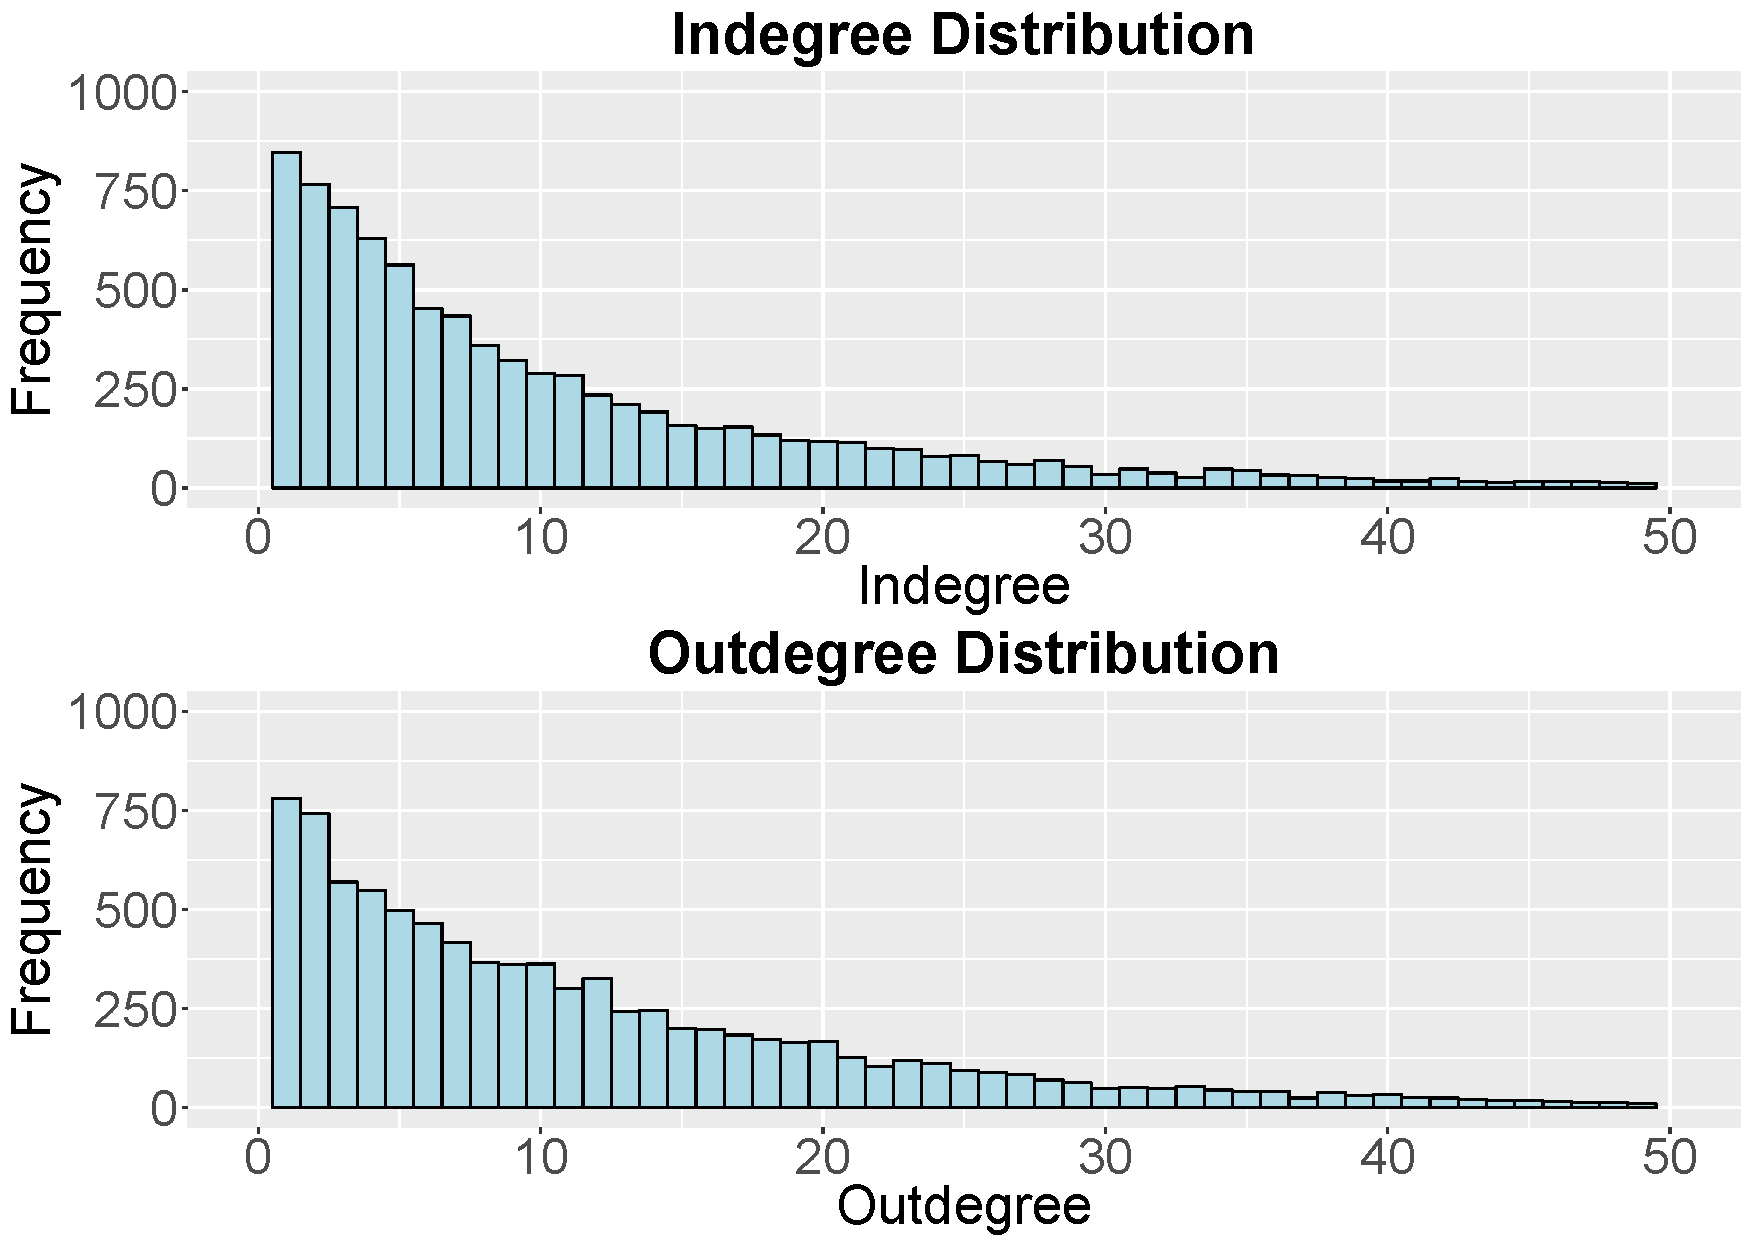
\includegraphics[scale=0.5]{degree_distribution}
\caption{The in- and outdegree distribution of the Supreme Court Citation Network from 1937 - 2001. There are cases with an indegree >50, but they are not captured in this figure.}
 \label{degree_dist}
\vspace{-.25cm}
\end{figure}

\begin{figure}[htp]
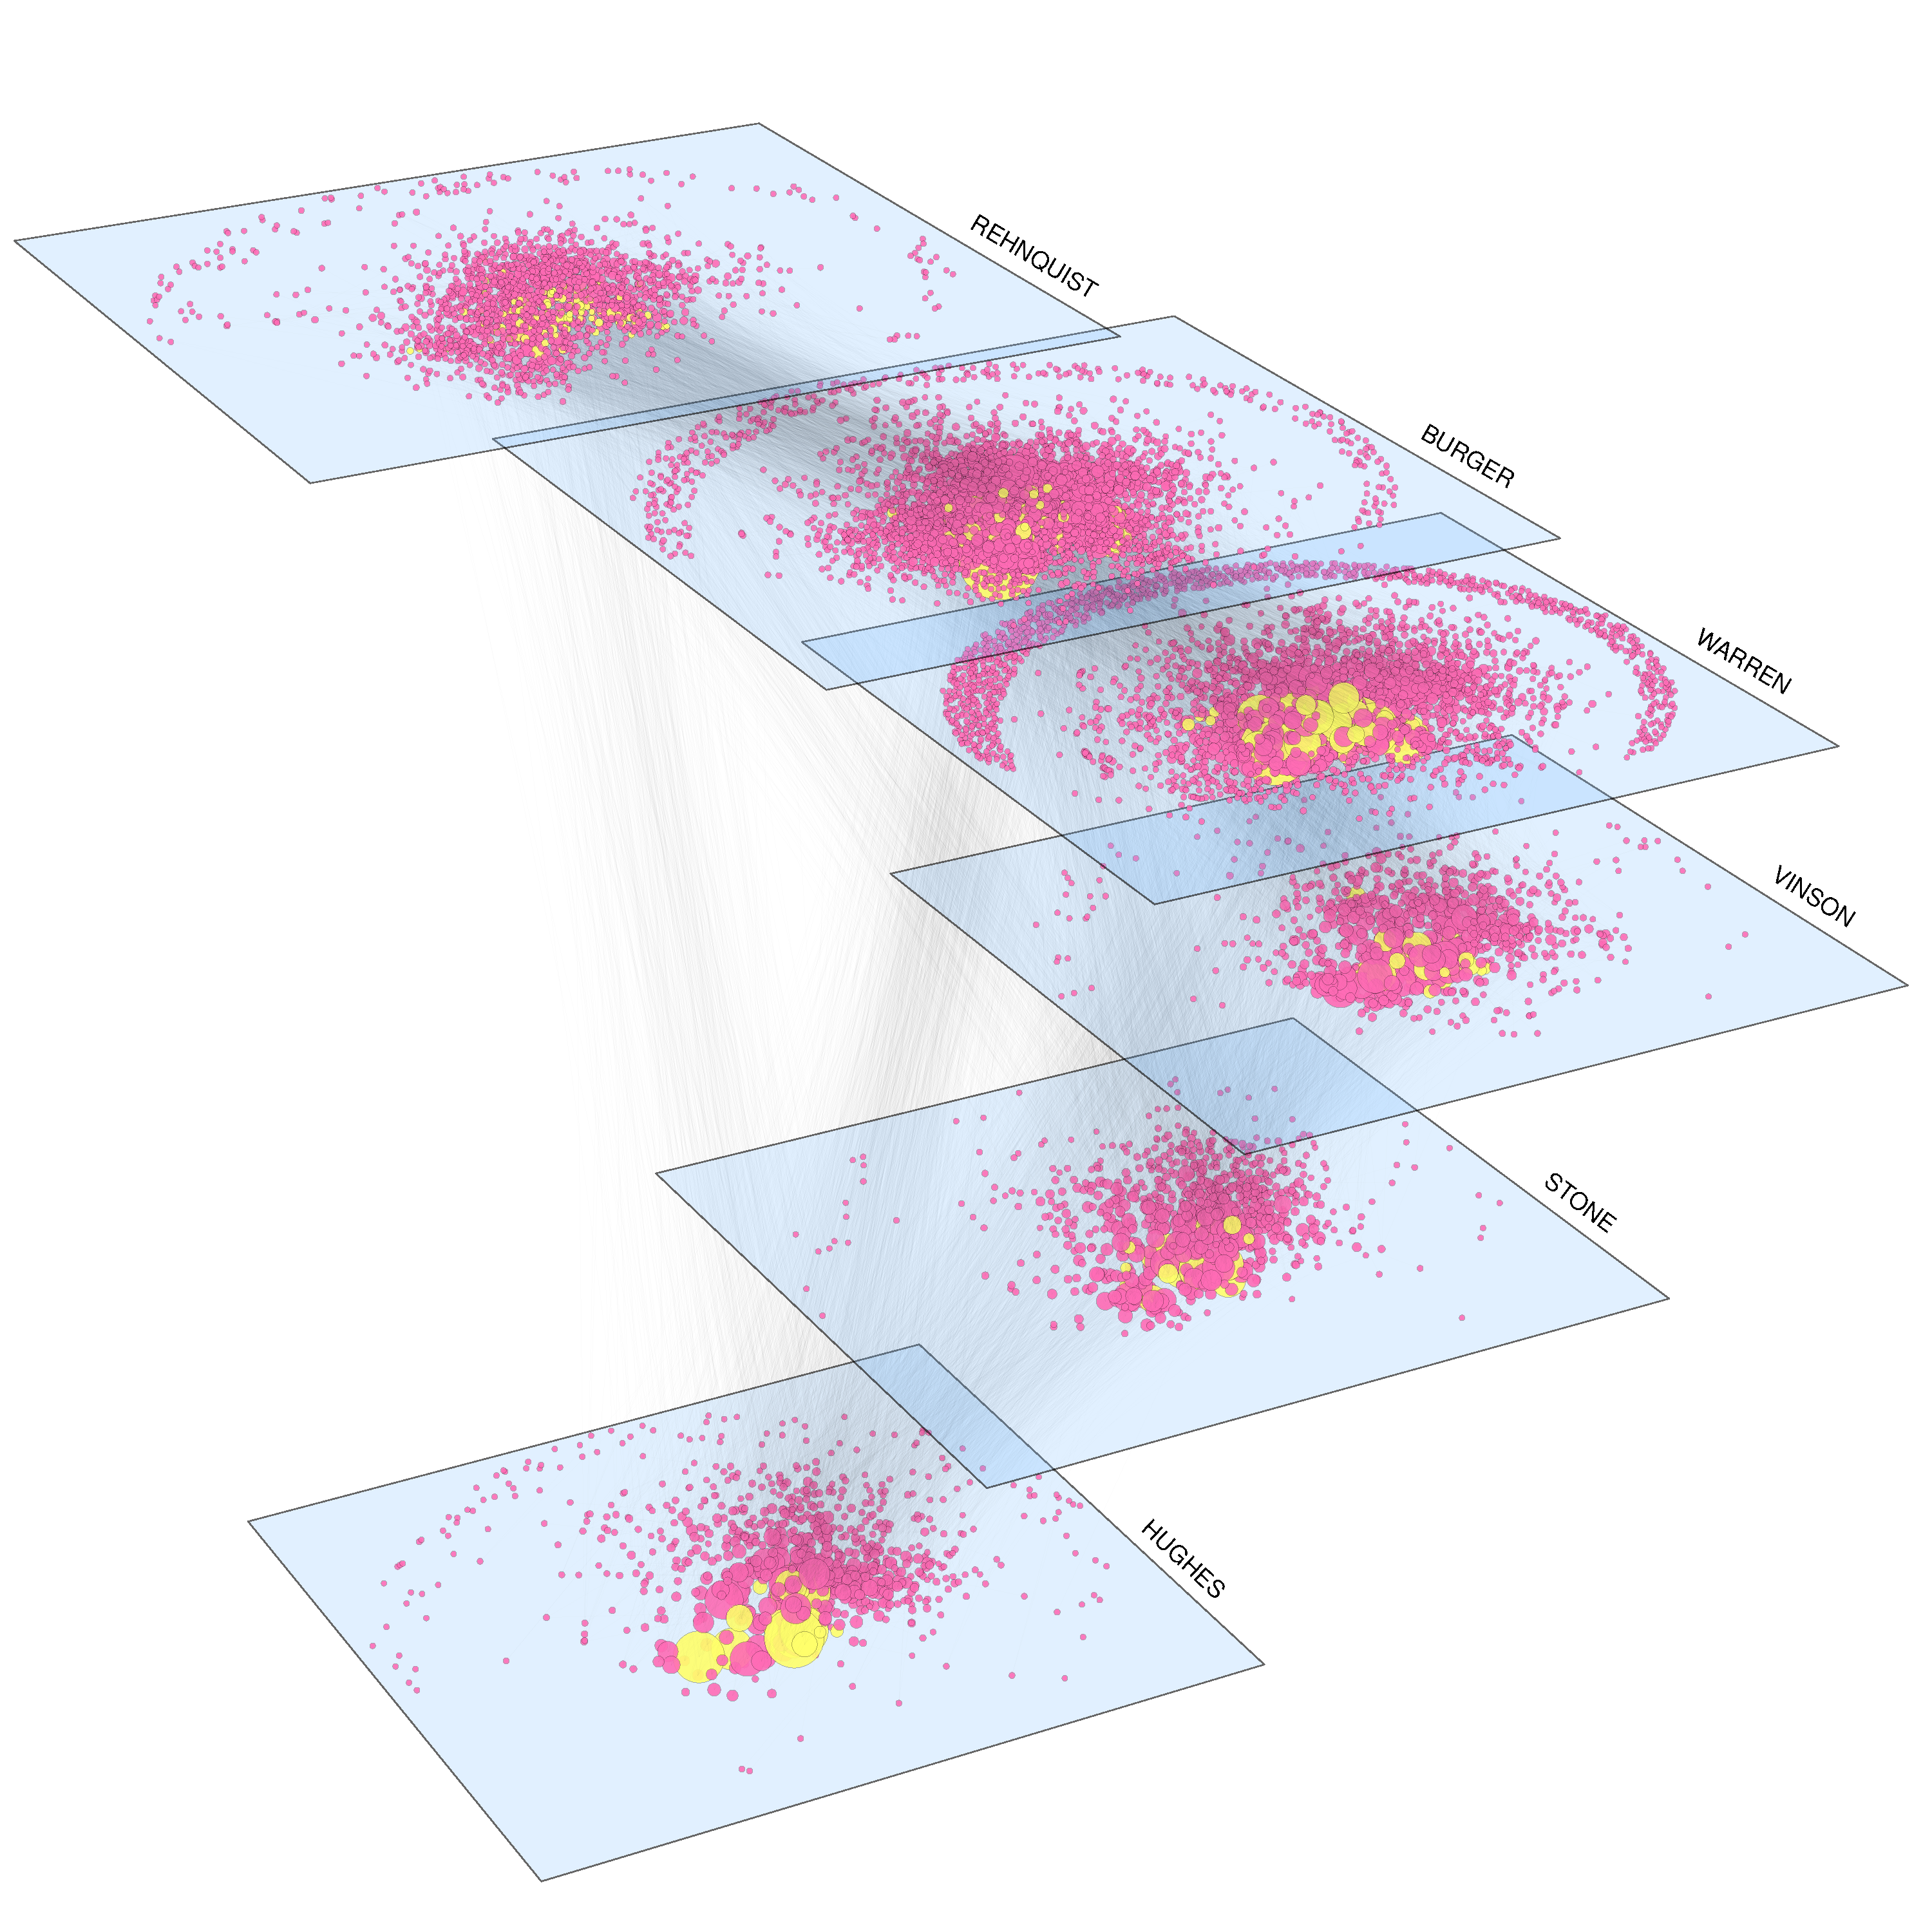
\includegraphics[scale=0.35,clip=true,trim=.5cm 0cm 0cm 2cm]{images/citations1}
\caption{ Supreme Court Citation Network, 1937?2001. Nodes are Supreme Court cases, with size based on incoming citations. Salient cases ({\em Oxford Guide}) are in yellow. Each network layer contains cases decided under a different chief justice. Because our data is temporally bound, cases for the Hughes and Rehnquist courts are not complete. }
 \label{fig:networkviz}
\vspace{-.25cm}
\end{figure}

  
\subsection{c-TERGM Results}



INTERPRETATION OF EFFECTS



\begin{table}[htp]
\footnotesize
\centering
\begin{tabular}{|
>{\columncolor[HTML]{EFEFEF}}l |l|l|l|l|} 
\hline
                                                   & \cellcolor[HTML]{EFEFEF}Estimate & \cellcolor[HTML]{EFEFEF}Lower Bound & \cellcolor[HTML]{EFEFEF}Upper Bound & \cellcolor[HTML]{EFEFEF}Significance \\
                                                    \hline
Edges                                              & -5.533                           & -5.733                              & -5.388                              & *                                    \\ \hline
Instar(2)                                          & 0.031                            & 0.027                               & 0.036                               & *                                    \\ \hline
Outstar(2)                                         & 0.022                            & 0.020                               & 0.032                               & *                                    \\ \hline
Mutual                                             & 3.316                            & 2.622                               & 3.983                               & *                                    \\ \hline
Triangle                                           & 1.490                            & 1.410                               & 1.560                               & *                                    \\ \hline
Martin Quinn Score                                 & 0.080                            & 0.022                               & 0.126                               & *                                    \\ \hline
Same Issue Area Homophily                          & 1.378                            & 1.313                               & 1.451                               & *                                    \\ \hline
Year Difference                                    & -0.077                           & -0.090                              & -0.064                              & *                                    \\ \hline
$(\text{Year Differnce})^2$                        & 0.0029                           & 0.0025                              & 0.0032                              & *                                    \\ \hline
Receiver Abs Diff MQ Score in Majority             & -0.030                           & -0.048                              & -0.014                              & *                                    \\ \hline
Receiver Number Justices in Majority               & -0.115                           & -0.135                              & -0.089                              & *                                    \\ \hline
Receiver  Sender Year                              & 0.0007                           & 0.0006                              & 0.0009                              & *                                    \\ \hline
Sender Same Issue Area 2                           & 0.162                            & 0.105                               & 0.217                               & *                                    \\ \hline
Sender Same Issue Area 3                           & -0.317                           & -0.403                              & -0.236                              & *                                    \\ \hline
Sender Same Issue Area 4                           & 0.497                            & 0.426                               & 0.570                               & *                                    \\ \hline
Sender Same Issue Area 5                           & 0.332                            & 0.174                               & 0.495                               & *                                    \\ \hline
Sender Same Issue Area 6                           & 0.527                            & 0.402                               & 0.635                               & *                                    \\ \hline
Sender Same Issue Area 7                           & 0.327                            & 0.251                               & 0.394                               & *                                    \\ \hline
Sender Same Issue Area 8                           & 0.076                            & 0.021                               & 0.129                               & *                                    \\ \hline
Sender Same Issue Area 9                           & 0.261                            & 0.209                               & 0.315                               & *                                    \\ \hline
Sender Same Issue Area 10                          & 0.369                            & 0.301                               & 0.432                               & *                                    \\ \hline
Sender Same Issue Area 11                          & -0.046                           & -0.233                              & 0.151                               &                                      \\ \hline
Sender Same Issue Area 12                          & 0.0073                           & -0.075                              & 0.089                               &                                      \\ \hline
Sender Same Issue Area 13                          & 0.381                            & 0.162                               & 0.564                               & *                                    \\ \hline
Sender Same Issue Area 14                          & 0.151                            & -0.019                              & 0.300                               &                                      \\ \hline
Receiver Same Issue Area 2                         & 0.231                            & 0.166                               & 0.300                               & *                                    \\ \hline
Receiver Same Issue Area 3                         & -0.101                           & -0.209                              & -0.006                              & *                                    \\ \hline
Receiver Same Issue Area 4                         & 0.516                            & 0.425                               & 0.612                               & *                                    \\ \hline
Receiver Same Issue Area 5                         & 0.351                            & 0.183                               & 0.534                               & *                                    \\ \hline
Receiver Same Issue Area 6                         & 0.461                            & 0.284                               & 0.628                               & *                                    \\ \hline
Receiver Same Issue Area 7                         & 0.361                            & 0.281                               & 0.437                               & *                                    \\ \hline
Receiver Same Issue Area 8                         & 0.153                            & 0.097                               & 0.221                               & *                                    \\ \hline
Receiver Same Issue Area 9                         & 0.279                            & 0.221                               & 0.346                               & *                                    \\ \hline
Receiver Same Issue Area 10                        & 0.492                            & 0.413                               & 0.570                               & *                                    \\ \hline
Receiver Same Issue Area 11                        & 0.247                            & 0.056                               & 0.411                               & *                                    \\ \hline
Receiver Same Issue Area 12                        & 0.339                            & 0.246                               & 0.430                               & *                                    \\ \hline
Receiver Same Issue Area 13                        & 1.060                            & 0.845                               & 1.239                               & *                                    \\ \hline
Receiver Same Issue Area 14                        & 0.557                            & 0.255                               & 0.793                               & *                                    \\ \hline
Instar(2) $\times$ Sender Year                     & -0.00025                         & -0.00034                            & -0.00017                            & *                                    \\ \hline
Outstar(2) $\times$ Sender Year                    & -0.00036                         & -0.00056                            & -0.00028                            & *                                    \\ \hline
Mutual $\times$ Sender Year                        & -0.010                           & -0.043                              & 0.029                               &                                      \\ \hline
Triangle $\times$ Sender Year                      & -0.0004                          & -0.0021                             & 0.0016                              &                                      \\ \hline
Martin Quinn Score $\times$ Sender Year            & -0.0025                          & -0.0035                             & -0.0013                             & *                                    \\ \hline
Same Issue Area $\times$ Sender Year               & -0.0058                          & -0.0076                             & -0.0043                             & *                                    \\ \hline
Year Difference $\times$ Sender Year               & 0.0004                           & 0.0002                              & 0.0007                              & *                                    \\ \hline
$\text{Year Difference}^2 \times$ Sender Year      & -0.000037                        & -0.000044                           & -0.000030                           & *                                    \\ \hline
MQ Score in Majority $\times$ Sender Year & 0.0013                           & 0.0009                              & 0.0017                              & *                                    \\ \hline
Justices in Majority $\times$ Sender Year   & 0.0029                           & 0.0023                              & 0.0035                              & *                                    \\ \hline
\end{tabular}
\caption{Bootstrapped MPLE Results for the time period $1937-2001$. A '*' indicates that the 2.5th and 97.5th quantile of the variable does not include '0' and as a result is statistically significant.}
\label{my-label}
\end{table}
\newpage


  \begin{figure}[H]
  \begin{tabular}{cc}
 (a) MQ Score Difference & (b) Ideological Breadth \\
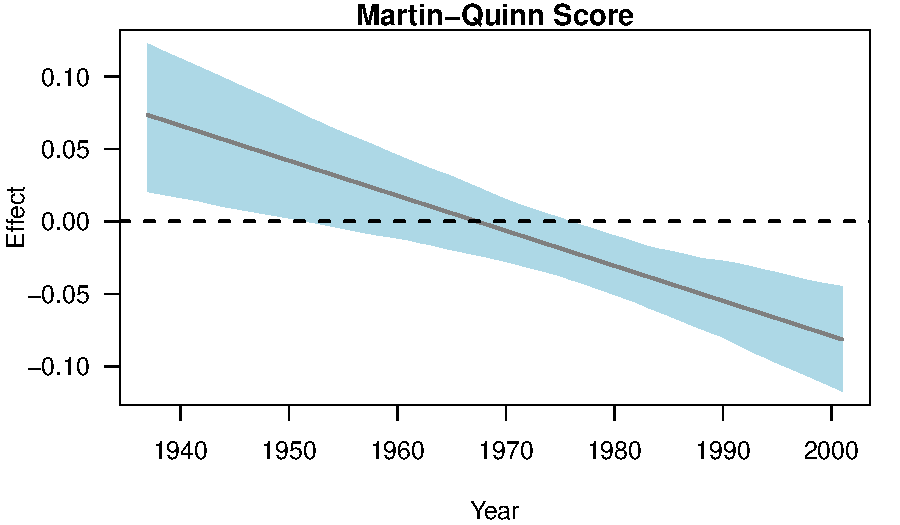
\includegraphics[width = 0.475\textwidth, trim= 0.1cm 1cm 0.5cm .45cm,clip=true]{images/mq_coef_trend.pdf} & 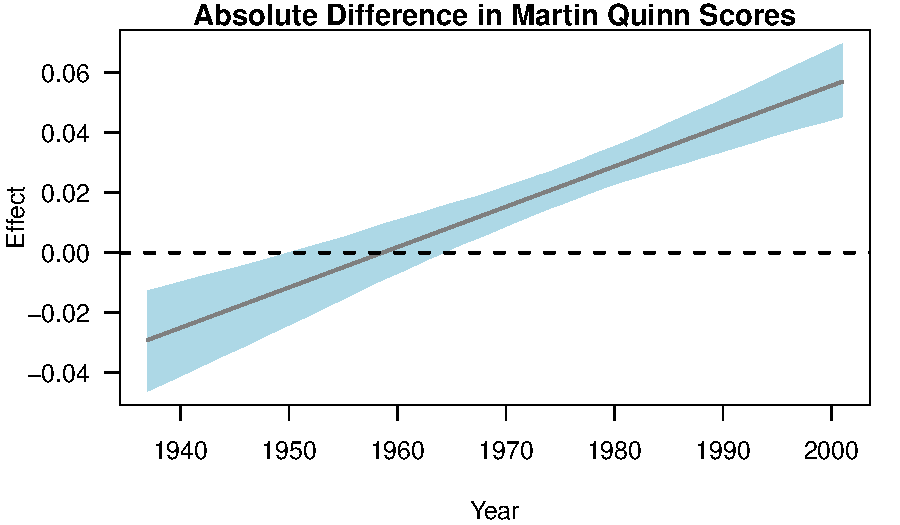
\includegraphics[width = 0.475\textwidth, trim= 0.1cm 1cm 0.5cm .45cm,clip=true]{images/absdiffmq_coef_trend.pdf} \\
 
  (c) Same Issue & (d) Majority Size \\
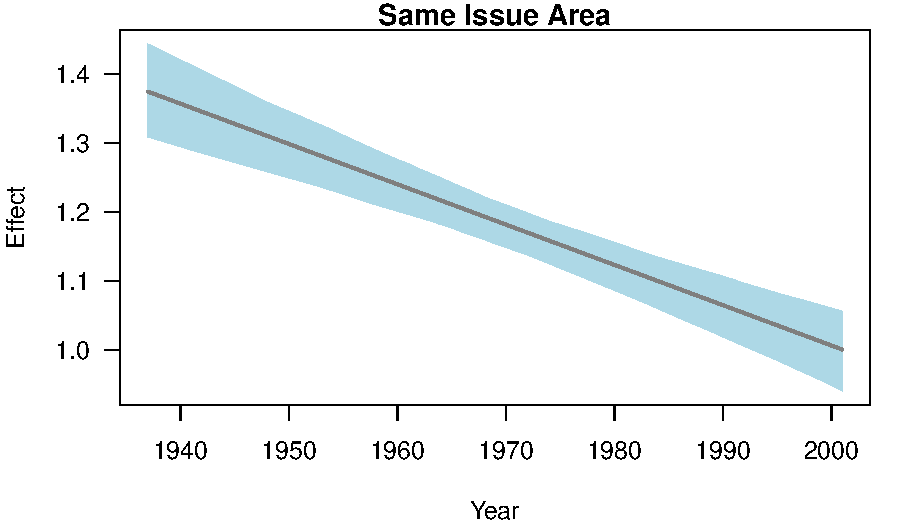
\includegraphics[width = 0.475\textwidth, trim= 0.1cm 1cm 0.5cm .45cm,clip=true]{images/sameissue_coef_trend.pdf} & 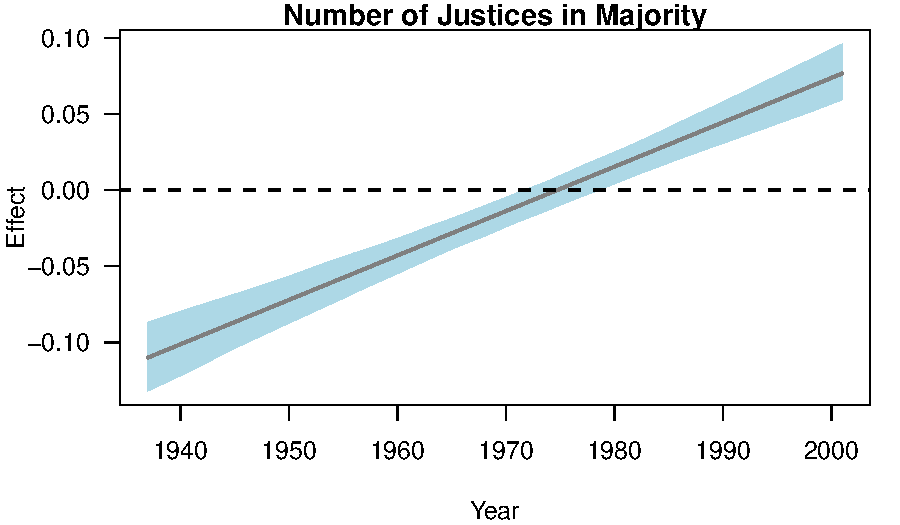
\includegraphics[width = 0.475\textwidth, trim= 0.1cm 1cm 0.5cm .45cm,clip=true]{images/numberjusticespro_coef_trend.pdf} \\
 
   (e) Reciprocity & (f) Transitivity \\
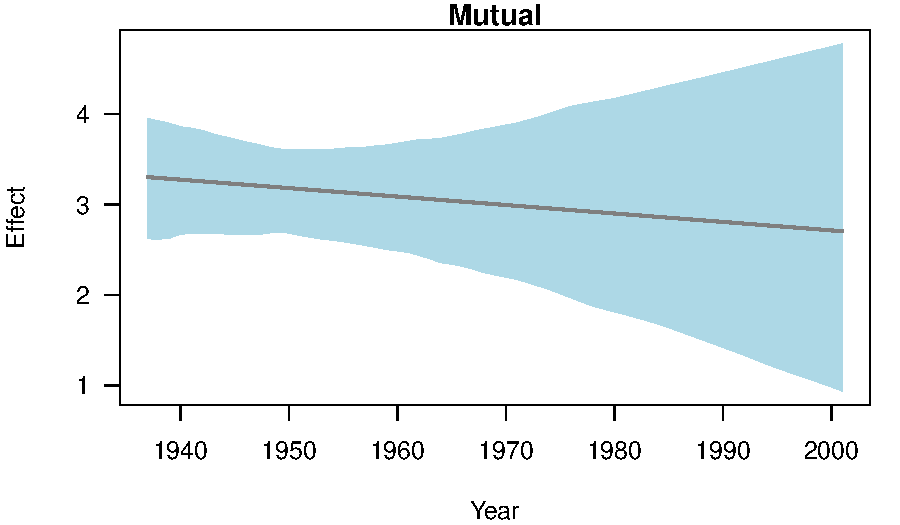
\includegraphics[width = 0.475\textwidth, trim= 0.1cm 1cm 0.5cm .45cm,clip=true]{images/mutual_coef_trend.pdf} & 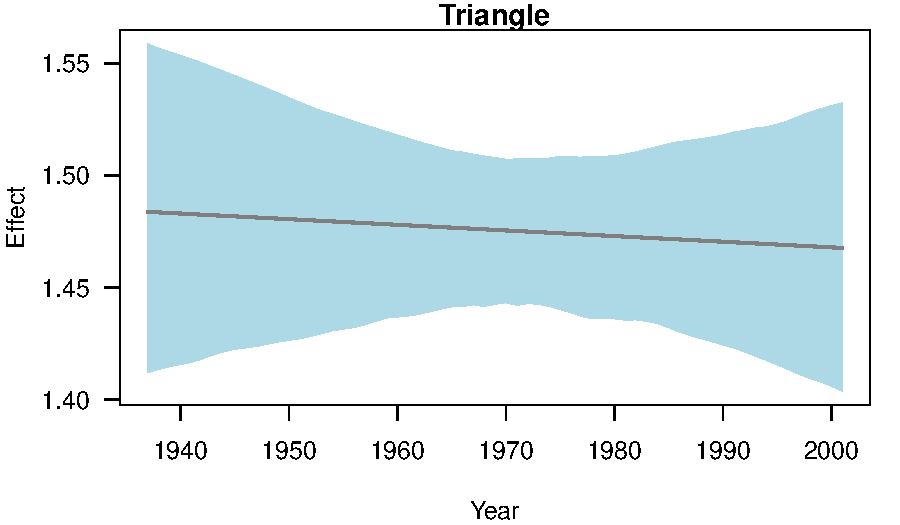
\includegraphics[width = 0.475\textwidth, trim= 0.1cm 1cm 0.5cm .45cm,clip=true]{images/triangle_coef_trend.pdf} \\
 
    (g) Activity & (h) Popularity \\
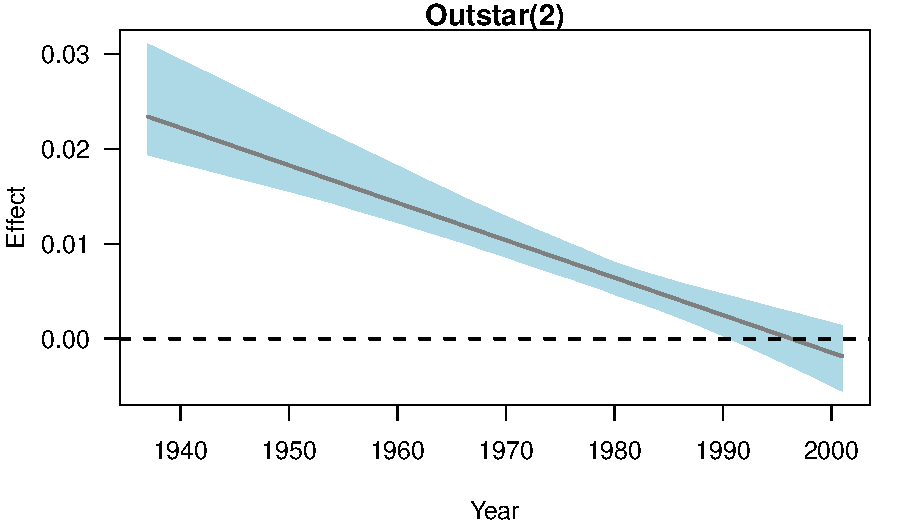
\includegraphics[width = 0.475\textwidth, trim= 0.1cm 1cm 0.5cm .45cm,clip=true]{images/o2star_coef_trend.pdf} & 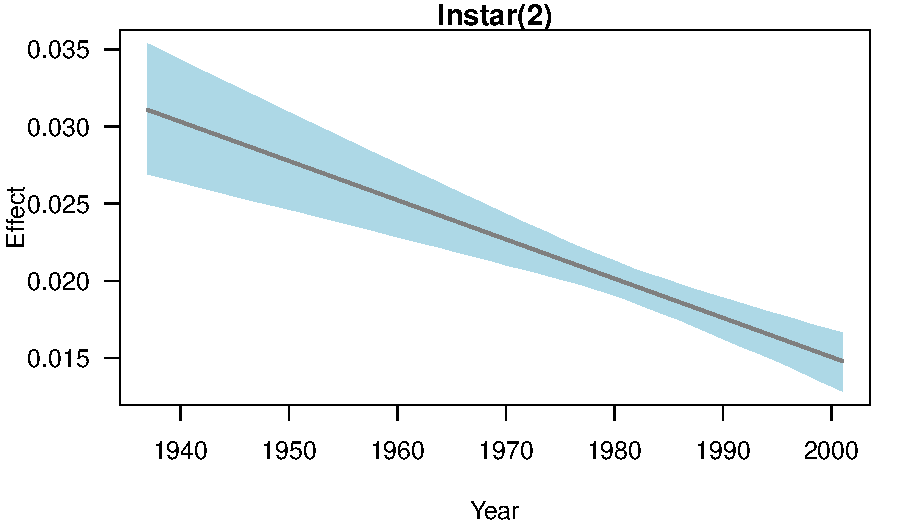
\includegraphics[width = 0.475\textwidth, trim= 0.1cm 1cm 0.5cm .45cm,clip=true]{images/i2star_coef_trend.pdf} \\
 
 
\end{tabular}
\caption{Effects}
 \label{fig:coeftrends}
\vspace{-.25cm}
\end{figure} 


\subsection{Predictive Performance}

Our case for studying legal citaions at the directed dyadic level hinges upon the contribution to modeling offered by incorporating network dependence. To quantify this contribution, we use out-of-sample prediction [CITES]. Predicting out-of-sample offers an unbiased and general purpose way to evaluate the contribution, in terms of model fit, of one or more terms/parameters in a model. Unlike in-sample measures of model fit, out-of-sample methods are highly robust in avoiding overfitting, and work when we cannot accurately calculate the value of the likelihood function, as in the current case. Out-of-sample prediction is a common way to evaluate methods for modeling ties in networks, and has recently been applied to TERGMs in particular [CITE PA AND IEEE].

In our prediction experiment we randomly split the directed dyads into an 80\% training set and a 20\% test set. The parameters of the model are estimated using the directed dyads in the training set, and the parameters are used to form the conditional probability of a tie for all of the directed dyads in the test set. Directed dyads for which the conditional probability of a tie exceeds 0.5 are predicted to be citations. The experiment is run with the full model, and with a model that excludes all of the dependence terms (i.e., all terms involving reciprocity, in and out stars, and triangles)---the independent dyads model. We run this experiment for 10 iterations. Predictive performance is evaluated with three common and related measures---precision (i.e., the proportion of predicted citations that are actually citations), recall (the proportion of actual citations that are predicted to be citations), and the F1 score (the harmonic mean of precision and recall). All three measures are bounded between 0 and 1, with higher scores indicating better performance.

\begin{table}[ht]
\centering
\begin{tabular}{rllll}
\hline \hline
& \multicolumn{2}{c}{Independent Model} & \multicolumn{2}{c}{Full Model} \\
  \hline
 & mean & range & mean & range \\ 
  \hline
precision & 0.5499 & (0.5384, 0.5619) & 0.8605 & (0.8526, 0.8666) \\ 
  recall & 0.0827 & (0.0811, 0.0843) & 0.5858 & (0.5817, 0.5891) \\ 
  F1 score & 0.1438 & (0.141, 0.1463) & 0.6971 & (0.6941, 0.7008) \\ 
   \hline \hline
\end{tabular}
\caption{The predictive performance of the directed dyadic models, over ten 80/20 train/test splits.}
\label{tab:prediction}
\end{table}


We see from Table \ref{tab:prediction} that, based on all three measures, the predictive performance of the model improves dramatically from adding the network dependence terms. The recall of the full model is particularly impressive, indicating that it recovers over half of the actual citations in the test set. This provides clear evidence that the full model, which includes covariates and network dependence terms, represents a more accurate and complete model of the process of citation formation in US Supreme Court opinions.

\section{conclusion}

MAJOR LIMITATION---DO NOT CONSIDER SIGN OF CASES


\bibliography{bib} 
\bibliographystyle{apsr}


\end{document}






















% Network Statistics
The c-TERGM is specified through 
the decision regarding which network statistics $h(\cdot)$ to incorporate. We include the following statistics for the Supreme Court citation network:
$$h_{edges}:\mathcal{C}(N)\to \mathbb{R}~~~, ~~~c(t) \to \sum_{i=1}^Nc_i(t)$$
the number of citations made at time $t$.  $h_{edges}$ is like an intercept, and models the expected value of any given edge.
$$h_{outstar}:\mathcal{C}(N)\to \mathbb{R}~~~, ~~~c(t) \to \sum_{j<i}^Nc_i(t)\cdot c_j(t) \cdot \sqrt{\dfrac{(t-a)(t-a-b)}{t^2}}$$
the number of weighted outstars occuring at time $t$. We argue that it should be more likely to cite more recent cases than cases that have been decided further in the past. For the weight 
$$w(a,b):= \sqrt{\dfrac{(t-a)(t-a-b)}{t^2}}$$
we define $a$ and $b$ as the elapsed time since case $i$ and $j$ have been introduced to the network.
$$h_{triangle}:\mathcal{C}(N)\to \mathbb{R}~~~, ~~~c(t) \to \sum_{j<i}^Nc_i(t)\cdot c_j(t) \cdot
c_j(t_{-i}) \cdot w(a,b)$$
where $c_j(t_{-i})$ indicates whether case $j$ was cited at the time case $i$ was introduced into the network. Just as for the outstar statistic, we include a weighting factor to favor more recent cases. \\[0.3cm]


%Change Statistic
The individual entries $c_i(t)$ can be taken as a manifestation of single Bernoulli variables $C_i(t)$. This interpretation allows the following calculation regarding the conditional distribution of $C_i(t)$:
%
\begin{eqnarray*}
\dfrac{P_{\theta}(C_i(t)=1 ~|~ C_i(t)^c=c_i(t)^c)}{P_{\theta}(C_i(t)=0 ~|~ C_i(t)^c=c_i(t)^c)} &=&
\dfrac{P_{\theta}(C_i(t)=1 ~,~ C_i(t)^c=c_i(t)^c)}{P_{\theta}(C_i(t)=0 ~,~ C_i(t)^c=c_i(t)^c)} \\
                           &=&\dfrac{P_{\theta}(C(t)= c_i^+(t))}{P_{\theta}(C(t)=c_i^-(t))}\\
                           &=&\dfrac{\exp(\theta^T \cdot h(c_i^+(t)~|~c(t-)))}{\exp(\theta^T \cdot h(c_i^-(t)~|~c(t-)))}\\
                           &=& \exp(\theta^T \cdot (h(c_i^+(t)~|~c(t-)) - h(c_i^-(t)~|~c(t-)))
\end{eqnarray*}
%
This implies the following equation:
%
\begin{equation}
\text{logit}(P_{\theta}(C_i(t)=1 ~|~ C_i(t)^c=c_i(t)^c))= \theta^T \cdot (h(c_i^+(t)~~|c(t-)) - h(c_i^-(t)~|~c(t-)))
\label{Logit}
\end{equation}
In the equation above the following notations were used:
%
\begin{itemize}
\item $c_i^+(t)$ emerges from $c(t)$, while assuming $c_i(t)=1$
\item $c_i^-(t)$ emerges from $c(t)$, while assuming $c_i(t)=0$
\item The condition $C_i(t)^c=c_i(t)^c$ is short for: $C_j(t)=c_j(t)$ for all $j\in \{1,\dots,N\}$ with $i \neq j$
\item The expression $(\Delta c_i)(t):=h(c_i^+(t)~|~c(t-)) - h(c_i^-(t)~|~c(t-))$ is called the \textit{change statistic}. The $k$th component of $(\Delta c_i)(t)$ captures the difference between citation networks $c_i^+(t)$ and $c_i^-(t)$ on the $k$th integrated statistic in the model
\end{itemize}



\section{Estimation}

% Pseudo Likelihood
\subsection*{Maximum Pseudo-Likelihood Estimator}
One can assume that the dyads are independent of each other, which means that
the random variables $C_i(t)$ inside the random vector $C(t)$ are independent of each other.
In this case, the equation (\ref{Logit}) reduces to
$$logit(P_{\theta}(C_i(t) = 1)) = \theta^T \cdot (\Delta c_i)(t)$$
This corresponds with the logistic regression approach, where the observations of
the dependent variables are simply edge values of the observed citation vector,
and the observations of the covariate values are given as the scores of every single
change statistic. Therefore, the resulting likelihood function is of the following form:
\begin{equation}
\text{lik}(\theta)= P_{\theta}(C(t)=c(t))= \prod_{i} \dfrac{ \exp \left(\theta^T \Delta(c_i)(t) \right)}{1+\exp \left(\theta^T \Delta(c_i)(t) \right)}
\label{PseudoLik}
\end{equation}

\subsection*{Maximum Likelihood Estimator}
The more rigorous technique is to estimate the parameters directly with the log-likelihood function derived from (\ref{ercm}), which has the following form:
%
\begin{equation}
\text{loglik}(\theta)=\theta^T \cdot h(c(t)| c(t-))-\log(\kappa(\theta))
\label{loglik}
\end{equation}
%
The problem resulting from estimating the parameters with (\ref{loglik}) is that the term
%
$$\kappa(\theta):= \sum_{c(t)^* \in \mathcal{C}(N)} \exp(\theta^T \cdot h(c(t)^*|c(t-)))$$ 
%
which sums up the weighted statistics of all possible binar vectors of length $N$, has to be evaluated. However, the cardinality of $\mathcal{C}(N)$ (\#$(\mathcal{C})=2^N$) is incredibly large and a direkt calculation of this sum is for already small $N$ not feasible. \\[0.3cm]
An solution for this limitation is based on the following consideration: Fix a vector of parameters $\theta_0 \in \Theta$ from the underlying parameter range $\Theta$ and compute for $\theta \in \Theta$ the expected value
%
\begin{eqnarray*}
\mathbb{E}_{\theta_0}\left[ \exp\left((\theta - \theta_0)^T \cdot \Gamma(C(t))\right) \right]&=& 
\sum_{c(t) \in \mathcal{C}(N)}\exp\left((\theta - \theta_0)^T \cdot \Gamma(c(t))\right)\cdot \mathbb{P}_{\theta_0}(C(t)=c(t))\\
&=& \sum_{c(t) \in \mathcal{C}(N)}\exp\left((\theta - \theta_0)^T \cdot \Gamma(c(t))\right)\cdot 
\frac{\exp(\theta_0^T \cdot \Gamma(c(t)))}{\kappa(\theta_0)}\\
&=& \frac{1}{\kappa(\theta_0)} \sum_{c(t) \in \mathcal{C}(N)}\exp\left(\theta^T \cdot \Gamma(c(t))\right)\\
&=&\frac{\kappa(\theta)}{\kappa(\theta_0)}
\end{eqnarray*}
%
This equation offers the following possibility: If one draws $L$ random vectors $c^{(1)}(t), \dots ,c^{(L)}(t)$ out of a distribution $\mathbb{P}_{\theta_0}$ appropriately, one gets with the law of big numbers and a big enough sample $L$ the following relation:
%
\begin{equation}
\frac{1}{L}\cdot \sum_{i=1}^{L}  \exp\left((\theta - \theta_0)^T \cdot \Gamma(c^{(i)}(t))\right)
~~\approx~~ \mathbb{E}_{\theta_0}\left[ \exp\left((\theta - \theta_0)^T \cdot \Gamma(C(t))\right) \right] = \frac{\kappa(\theta)}{\kappa(\theta_0)}
\label{konver}
\end{equation}
%
This approximate can then be used to approximate the log likelihood function.\\[0.4cm]
Next, we will discuss how a sufficient number of suitable drawings $c^{(1)}(t), \dots ,c^{(L)}(t)$ can be sampled from the distribution $\mathbb{P}_{\theta_0}$. \\
For this purpose, the Markov Chain Monte Carlo (MCMC) methods can be used.
\subsection*{Gibbs sampling for the ERCM}
To be able to compute the approximate likelihood function one needs a sufficiently large number of random vectors from the distribution $\mathbb{P}_{\theta_0}$. Snijders \citet{Snijders.2002b} introduces an approach to sample random networks for the ERGM framework by using \textit{MCMC methods}. We adapt this approach for sampling appropriate binary vectors for the ERCM. \\[0.4cm]
\textit{Gibbs sampling}\\
%Choose any vector $c^{(0)}(t) \in \mathcal{C}(N)$ (e.g. observed vector). Afterwards, the length $L$ of the respective sub-sequence is determined. For $k \in \{0,...,L-1\}$ execute the following steps recursively (here the vector in its $k$th iteration is denoted as $c^{(k)}(t)$):\\

\begin{algorithm}[H]
 Choose any vector $c^{(0)}(t) \in \mathcal{C}(N)$ (e.g. observed vector)\\
 \For{i in 1:N}{
  Compute $\pi:= \cfrac{\exp(\theta^T\cdot \Delta(c_i)(t))}{1+\exp(\theta^T\cdot \Delta(c_i)(t))}$\\
  Draw a random number Z from Bin(1,$\pi$)\\
  \eIf{Z=1}{
   set $c^{(k+1)}_i = 1$ and $c^{(k+1)}_j=c^{(k)}_j$, if $i\neq j$
   }{
   set $c^{(k+1)}_i = 0$ and $c^{(k+1)}_j=c^{(k)}_j$, if $i\neq j$
  }
 }
 Start all over using $c^{(k+1)}$\\[0.3cm]
 \caption{Simulation of vectors of $\mathbb{P}_\theta$ using Gibbs sampling}
\end{algorithm}
\vspace{0.5cm}
%\begin{enumerate}
%\item Randomly choose a number $i \in \{1,\dots, N\}$
%\item Compute using the likelihood the value 
%$$\pi:= \mathbb{P}_{\theta}(C_{i}(t)=1 | C_{i}^c(t)=(c_{i}^{(k)}(t))^c)=\cfrac{\exp(\theta^T\cdot \Delta(c_i)(t))}{1+\exp(\theta^T\cdot \Delta(c_i)(t))}$$
%\item Draw a random number $Z$ from Bin$(1, \pi)$. %If
%\begin{itemize}
%\item $Z=0$, define $c^{(k+1)}(t)$ via
%$$c_{p}^{(k+1)}(t)=\begin{cases}
%0& \text{if}~ p=i \\
%c_{p}^{(k)}(t) &\text{if}~ p \neq i 
%\end{cases}$$
%\item $Z=1$, define $c^{(k+1)}(t)$ via
%$$c_p^{(k+1)}(t)=\begin{cases}
%1& \text{if}~ p=i \\
%c_p^{(k)}(t) &\text{if}~ p \neq i 
%\end{cases}$$
%\end{itemize}
%\item Start at step 1 with $c^{(k+1)}(t)$.
%\end{enumerate}
\noindent Using the depicted algorithm, a sequence of random vectors $c^{(0)}(t),...,c^{(L)}(t)$ can be simulated. Since the orignial vector was chosen randomly and the first simulated vectors are very dependent on the chosen mvector (only one entry is changed per iteration!), usually the first $B$ vectors, where $N \ll B \ll L$, are discarded as the so called \textit{Burn-In}.
\subsection*{Metropolis Hastings for the ERCM}\label{networksimulation}
Choose any vector $c^{(0)}(t) \in \mathcal{C}(N)$ to start with (e.g., the observed vector). For $k \in \{0,...,L-1\}$ recursively proceed as follows:\\
\begin{enumerate}
\item Randomly choose a number $i\in \{1,\dots, N\}$
\item Compute, using the equation (\ref{Logit}) the value
$$\pi := \dfrac{\mathbb{P}_{\theta}(C_{i}(t) \neq c_{i}^{(k)}(t) ~| ~C_i(t)^c=c_i(t)^c)}{\mathbb{P}_{\theta}(C_{i}(t) = c_{i}^{(k)}(t) ~| ~C_i(t)^c=c_i(t)^c)}$$
\item Define $\delta:= \min\{1, \pi\}$ and draw a random number $Z$ from Bin$(1, \delta)$. If
\begin{itemize}
\item $Z=0$, let $c^{(k+1)}(t) := c^{(k)}(t)$ 
\item $Z=1$, define $c^{(k+1)}(t)$ as
$$c_{p}^{(k+1)}(t)=\begin{cases}
1-c_{p}^{(k)}(t)& \text{if}~ p=i \\
c_{p}^{(k)}(t) &\text{if}~ p \neq i 
\end{cases}$$
\end{itemize}
\item Start at step 1 with $c^{(k+1)}(t)$.
\end{enumerate}
The first $B \ll L$ vectors are discarded as Burn-In.




First, as these arcs are observed patterns of behaviour, they can be used to infer latent characteristics of nodes or the relations between nodes that produced them \citep{batagelj2003efficient}. Moreover, since each judgment is embedded in the broader network of citations, which influences the judgment beyond the characteristics of the two directly linked documents, inferences about the neighborhood of these two documents are possible as well. A common application of this general logic is to obtain local or global network indices, such as Kleinberg centrality at the node level \citep{kleinberg1999authoritative,fowler2007network} or global hierarchy \citep{mones2014universal}, then use them to draw conclusions about networks or compare networks across contexts such as time periods \citep[e.g.][]{vazquez2001statistics,fowler2008authority,greenberg2009citation,lupu2012precedent,lupu2013strategic,dawson2014current,jaffe2017patent}.
	
	Still within the category of using observed network constellation to make inferences about components of the system, identification of communities using methods for clustering, such as modularity maximization \citep[e.g.][]{kajikawa2007creating,shibata2011detecting,chen2010community} and stochastic block modeling \citep{jo2009citing}; and subnetwork identification \citep[e.g.][]{batagelj2017emergence} have been used to analyze relevance of topics within an academic field or to determine trends in technological advancement \citep{verspagen2007mapping,erdi2013prediction}. Main path analysis \citep{hummon1989connectivity}, which determines the main path through an acyclic network, is a particularly useful way to examine trends as it allows researchers identify structures of knowledge flow. Other methods include classifying documents into groups based on similarities in their citation profiles of cites over time, which can be examined as a function of time to see if there are temporal patterns \citep{leicht2007large}. The identification of communities is often coupled with classification of these communities by the researcher using historical knowledge. 


	\section{Extra Notes}
	This section contains some of the extra notes I cut out from the draft that might be useful.
	\subsection{Broader definitions of citation networks}
	More broadly, citation networks can have as nodes the document producers, including scientists \citep{ji2016coauthorship}, judges \citep{landes1998judicial}, journals \citep{rice1988citation}, or aggregated units \citep{gelter2012networks,pan2012world}. In these cases, which are essentially exercises in aggregation, the resulting network can take on different characteristics such as weighted or cyclic edges. Other networks derived from the raw citation network is the co-citation or co-cited-by networks whereby two documents are connected if they co-cite or are co-cited by another document \citep{van2005reference}.
	
	\subsection{Weighted edges and multiplexity}
	Recognition, and subsequent quantification, of different levels of complexity in citation arcs allows for a host of advancements in citation network analysis. Weights can indicate relevance \citep{liu2014citations} or be used to incorporate the temporal dimension into citation networks \citep{fujita2014detecting}. Moving to multiplexity leads to further advancements. For example, \citet{greenberg2009citation} accounted for level of support and through simulations based on arc typed switching demonstrated how citation bias against critical articles yielded differences in beliefs within a medical discipline. \citet{bommarito2010distance} argued that articles contain different types of information and accounting for the specific piece of information that resulted in the cite can yield clustering that are more interpretable. In all cases however, substantial work has to be done into reclassifying the weightedness or multiplexity of citation arcs \citep{zhang2007semantics}.
	
	\subsection{Misc. notes}
	\begin{itemize}
		\item To control for age, \citet{clough2015transitive} propose transitive reduction of citation networks (i.e. removal of redundant information ties) as it will primarily remove citation arcs that are disparate in age.
		\item Most citation networks are directed acyclic graphs, but not all. Different versions of the same document can also cause problems (such as strong network components). The ``preprint transformation'' is a solution to small strong components \citep{batagelj2017emergence}.
		\item Date of publication can be assigned as level to nodes in acyclic networks \citep{batagelj2017emergence}. Depending on the citation network at hand, temporal ordering can be difficult, as documents can share publication dates. To overcome this, begin each iteration by sampling from one of the possible orderings. \citep{carstens2016topology}.
	\end{itemize}
	
	\begin{figure}[H]
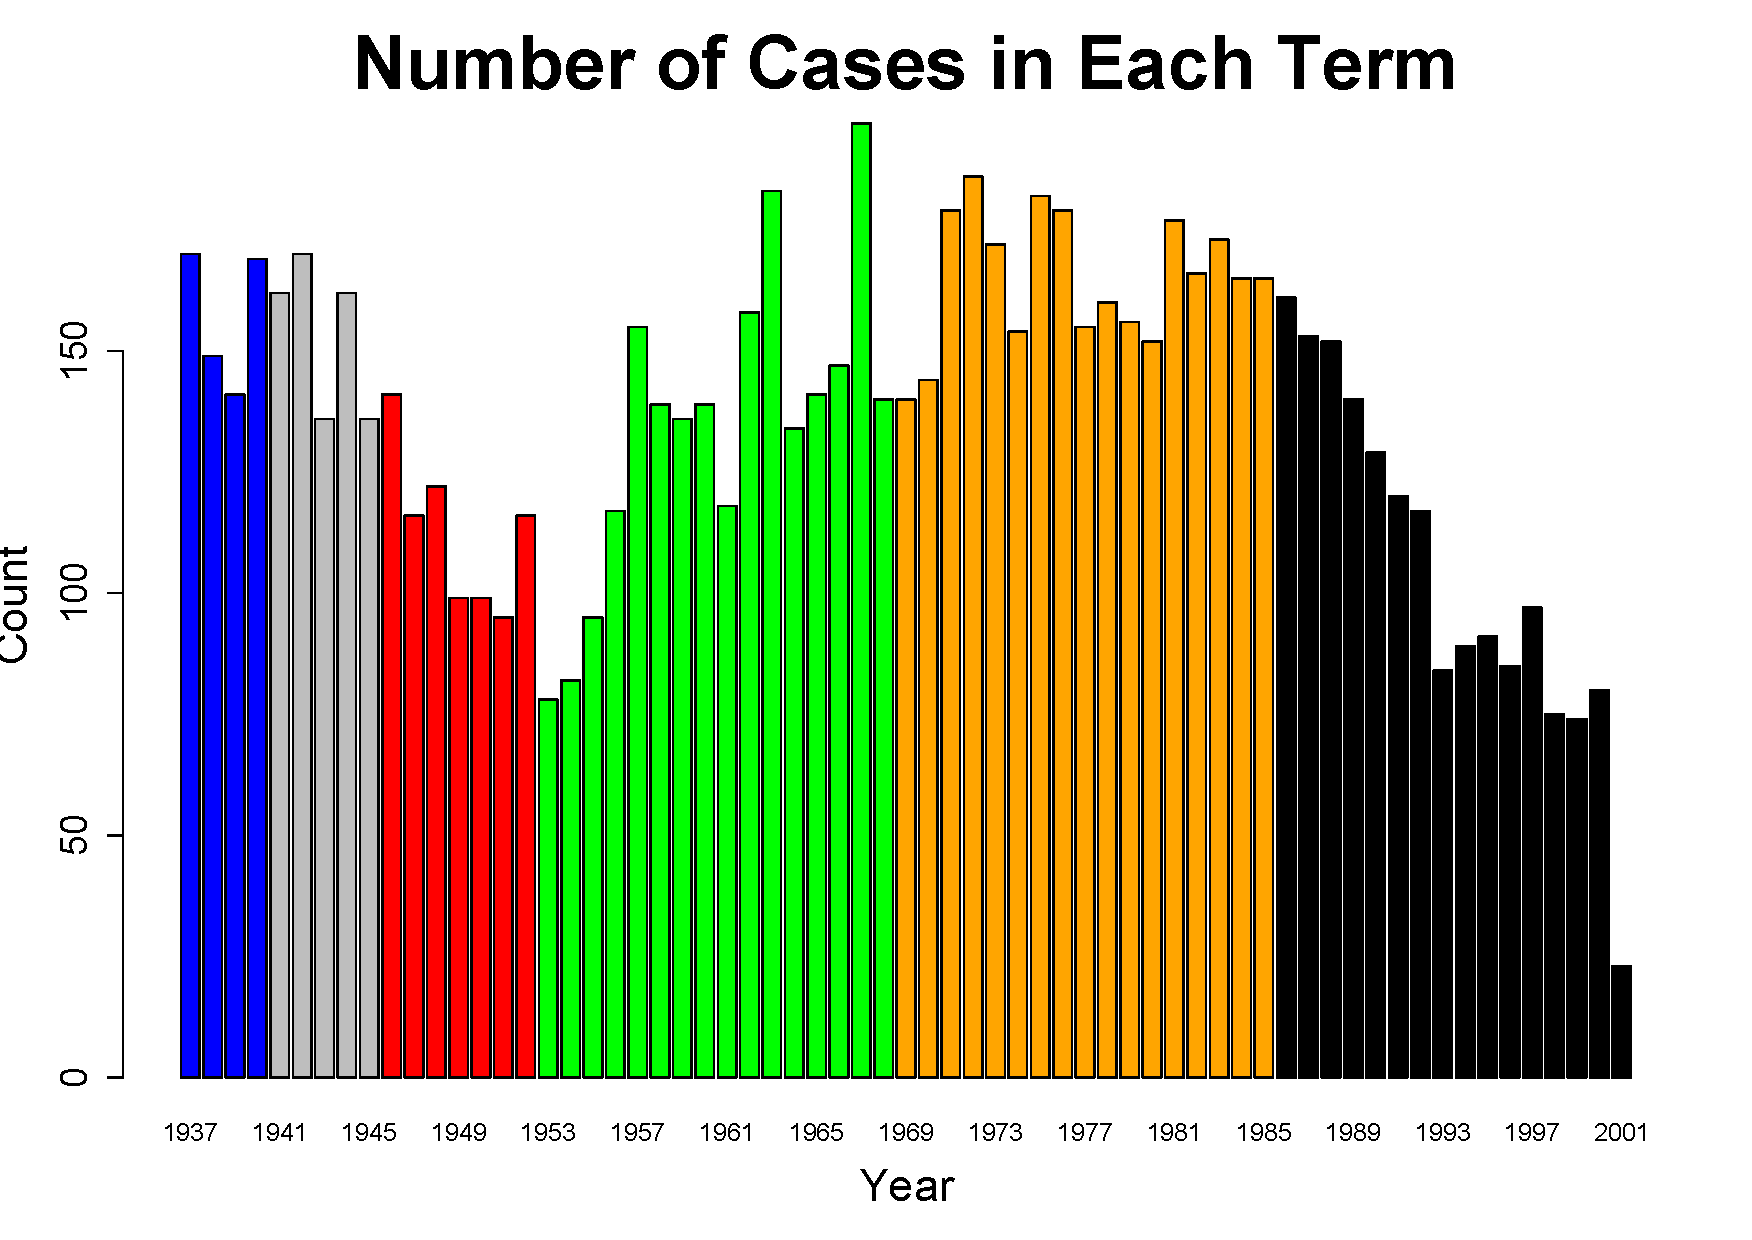
\includegraphics[scale=0.5]{number_cases}
\caption{Number of cases in each term. Different colors indicate different chief justices.}
 \label{number_cases}
\vspace{-.25cm}
\end{figure}  
  
 \begin{figure}[H]
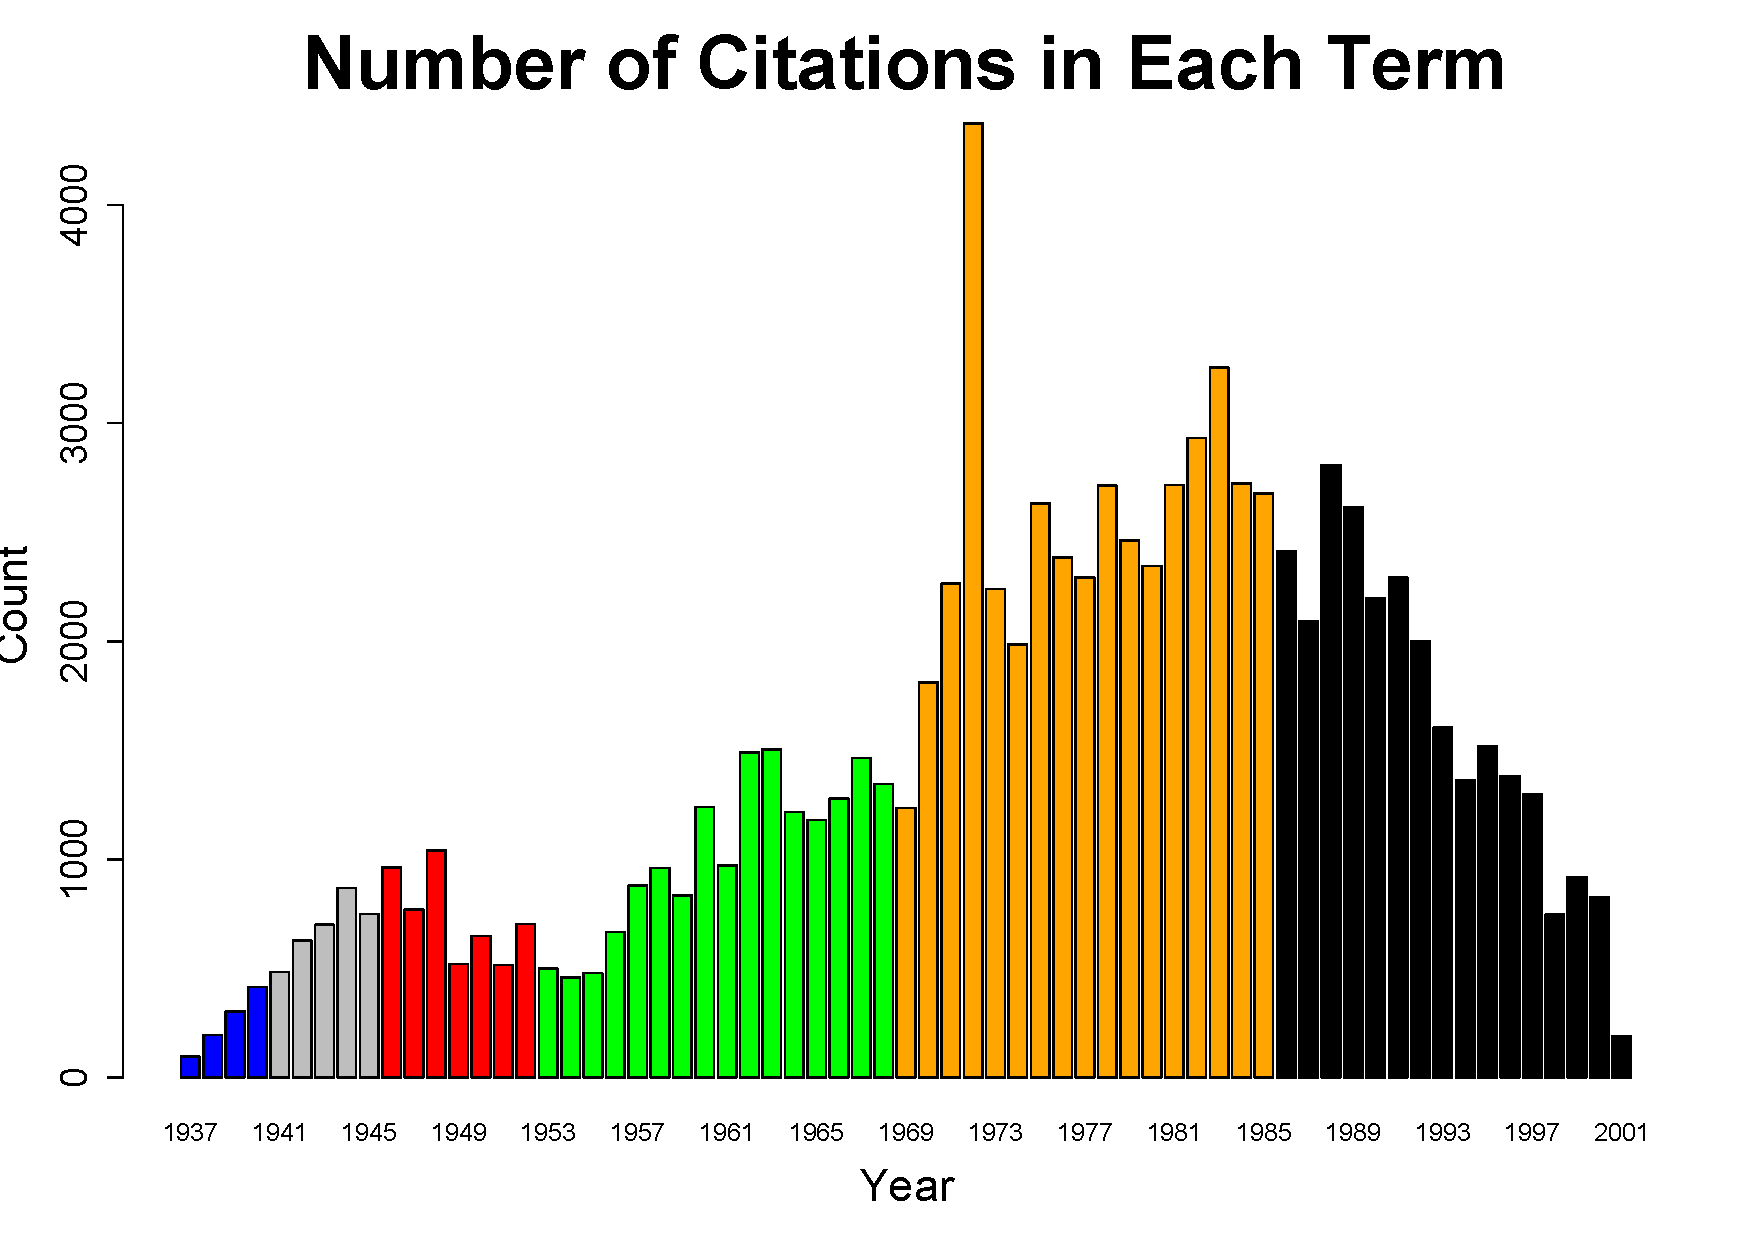
\includegraphics[scale=0.5]{number_citations}
\caption{Number of citations for the 1937-2001 time period. Citations for cases prior 1937 are not considered in this figure. Different colors indicate different chief justices.}
 \label{number_citations}
\vspace{-.25cm}
\end{figure}  
  
  \begin{figure}[H]
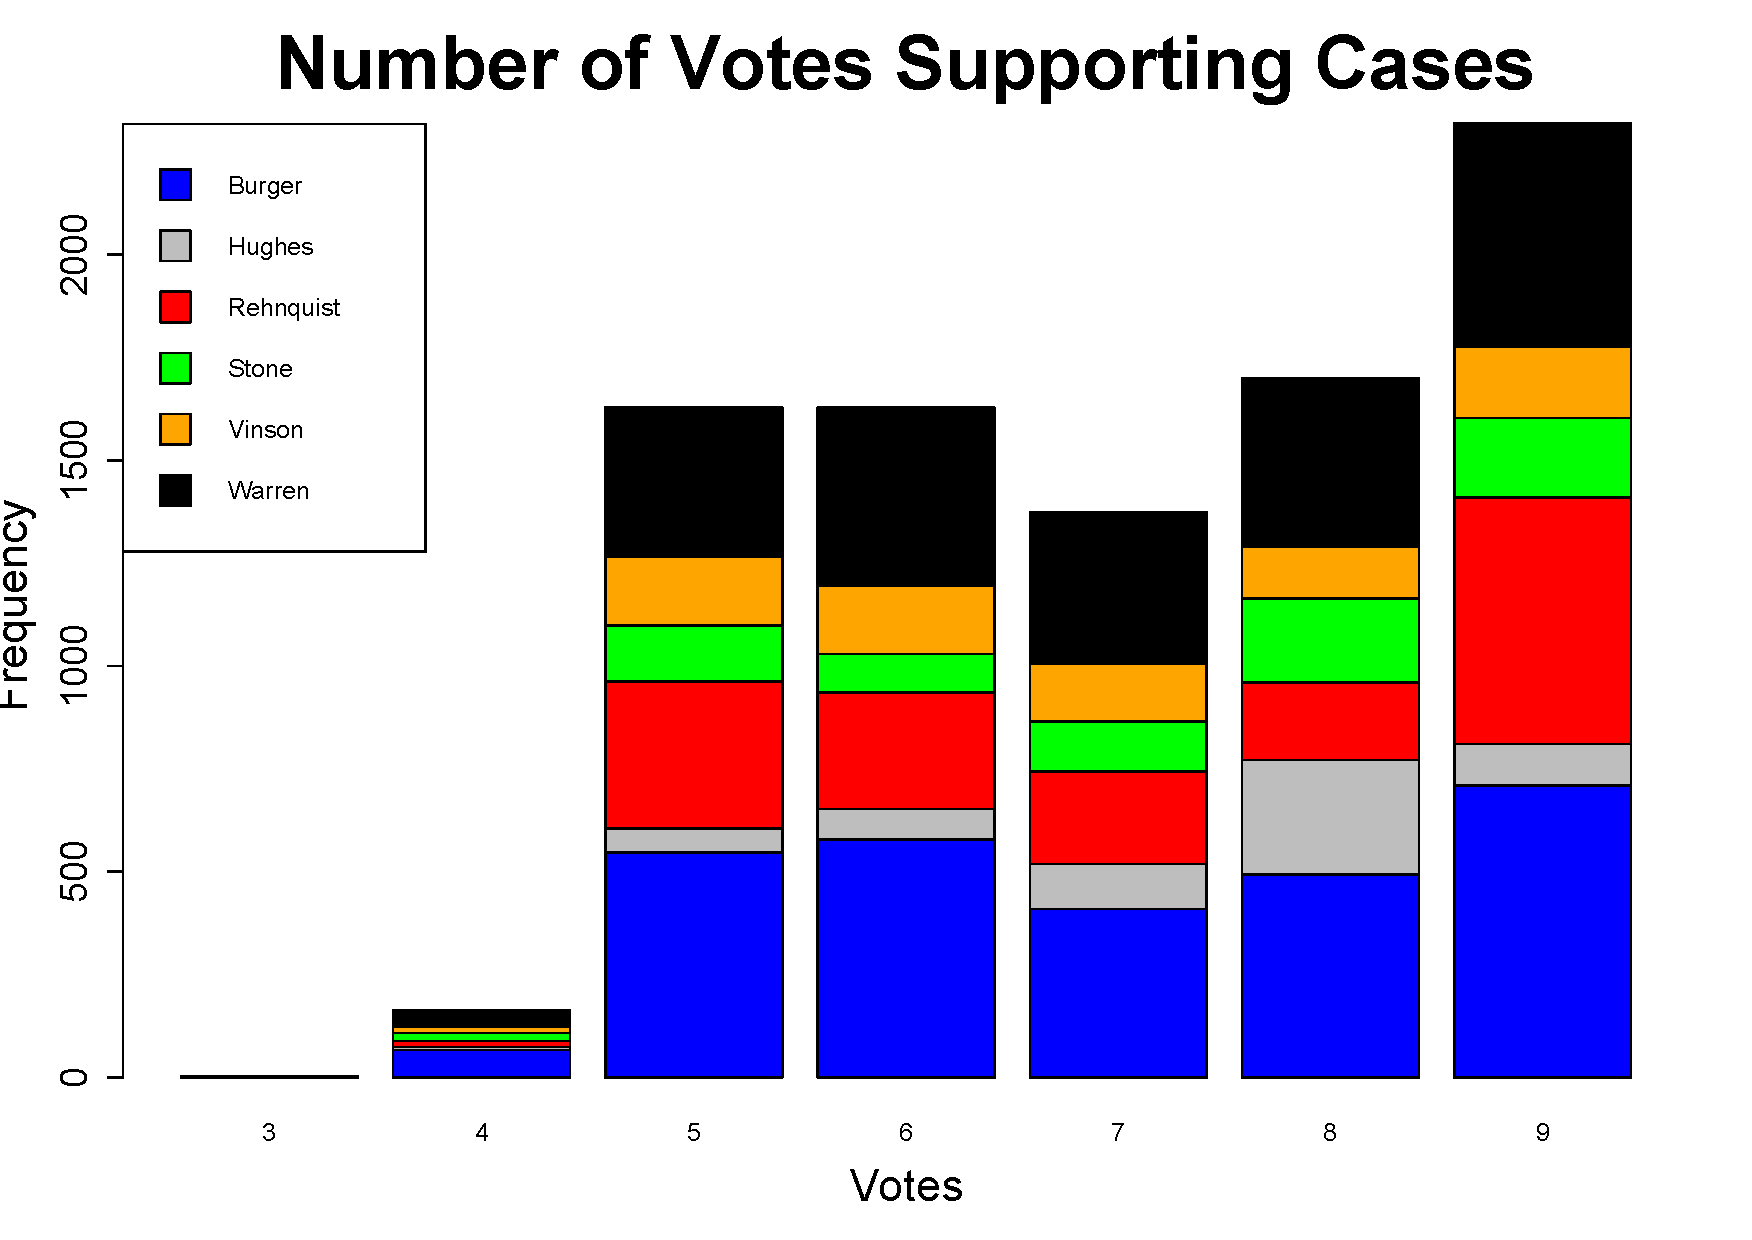
\includegraphics[scale=0.5]{number_votes_supporting}
\caption{Number of Votes that were supporting cases between 1937-2001. Different colors indicate terms with different chief justices. }
 \label{number_supporting}
\vspace{-.25cm}
\end{figure}  
  
\newpage 

